\documentclass{article}
\usepackage[utf8]{inputenc}
\usepackage[left=2.5cm,right=2.5cm,top=2.5cm,bottom=2.5cm]{geometry}

\usepackage{notes2bib}
\usepackage{amsmath}
\usepackage{amssymb}
\usepackage{hyperref}
\usepackage{graphicx}

\usepackage{epstopdf}
\usepackage{epsfig}

\usepackage{paralist} % inline list

\usepackage{amsthm} % theorem and definition
\newtheorem{mydef}{Definition}
\newtheorem{exmp}{Example}

\usepackage{algorithm2e}
\usepackage{algorithmic}
% \usepackage{algorithm}

\usepackage{tikz}
\usepackage{xytree}

\usepackage{color}

\usepackage{hhline}
\usepackage{float}
\restylefloat{table}

\usepackage{bm}
\newcommand\abs[1]{\left\lvert #1 \right\rvert}

\title{Mid-term Thesis Report\\High-level image interpretation using logical and morphological approaches}
\author{Yifan YANG}
\date{\parbox{\linewidth}{\centering%
  \today\endgraf\bigskip
  Advisors: Jamal ATIF, Isabelle BLOCH\endgraf\bigskip
  Thesis started in October 2013}}

\begin{document}

\maketitle
\section{Introduction}
% for automatic image understanding
 High-level semantics extraction from an image is an important research area  in artificial intelligence.
 Many related fields like image annotation, activity recognition and  decision-support systems take advantage of semantic content.
 Recognition of perceptual objects and scene understanding, which translate low level signal information into meaningful semantic information, belong to one of the fundamental abilities of human beings.
 As advanced as AI has become, it still remains a big challenge for computers to accomplish complex understanding tasks as humans do.
 Digital image itself is a numerical representation which does not represent explicitly semantic information. 
 Prior knowledge is intensively used by experts who interpret visually an image. It should then also be used by machines to associate semantics with the image.  
However, image interpretation still faces some difficulties, one of which is how to accurately associate perceptual data with appropriate concepts. Without an expert knowledge,
such a link is difficult to be established. This relation between visual percepts and high-level linguistic expression is called \textit{semantic gap}~\cite{hudelot2008spatial}.
 In this work, beyond a single object understanding based on low level features such as color and shape, we focus on a complex description which relies on context information like spatial relations
 between diverse objects as well as prior knowledge on the application domain. 
 For instance, in the context of medical applications, the understanding task can be formulated as giving an abstract description of a pathological brain volume, such as in Figure~\ref{fig:patho_brain}. 
  According to different levels of anatomical prior knowledge on brain pathology, two possible descriptions could be given:
 \begin{itemize}
  \item an abnormal structure is present in the brain,
  \item a peripheral non-enhanced tumor is present in the right hemisphere.
 \end{itemize}
 In this thesis, a high-level interpretation is regarded as an explanation of what we have seen in the image.
 This process is a backward-chaining inference based on  prior knowledge to link the abstract description and the observed context of the scene.
  \begin{figure}[h]
  \centering
   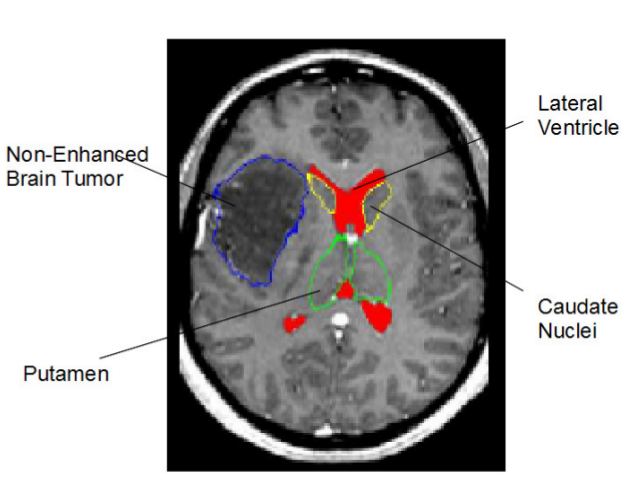
\includegraphics[scale=.2]{./figures/patho_brain.png}
   \caption{\label{fig:patho_brain} A slice of a pathological brain volume (MRI acquisition), where some structures are annotated.}
 \end{figure} 
\subsection{Problem formulation}
According to the objective pointed out in the introduction, our aim is to extract high-level semantic information from a given image and translate it at a linguistic level.
Concretely, we are interested in the interpretation of cerebral images with tumors. The high-level information corresponds to the presence of diverse types of pathologies
 as well as descriptions of brain structures and spatial relations among them in a brain image. 
 In the context of this thesis, the decision process is modeled as an abductive reasoning~\cite{aliseda1997seeking} using a logical formalism, 
 which is an inference mechanism from facts to explanations.
The objective of this thesis is to build a generic logic-based formalism as well as  to develop an appropriate reasoning process for image interpretation, 
 allowing us to extract a set of suitable candidates as potential hypotheses for a given image and to select the ``best'' one according to a defined criterion.  
 In image interpretation, spatial relationships are important when objects of similar appearance are present in the image, especially in magnetic resonance imaging (MRI).
 Such relationships have then to be included in the representation and in the reasoning process.

\begin{figure}[h]
  \centering
   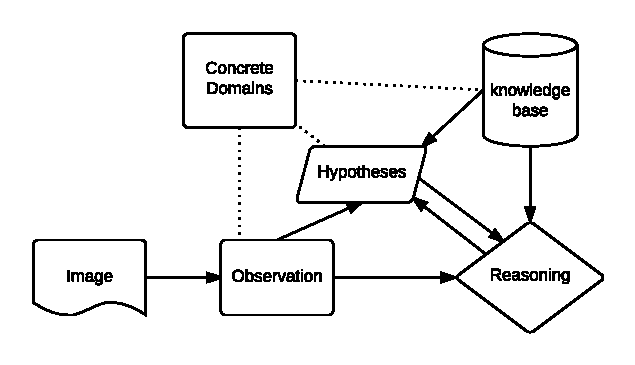
\includegraphics[scale=.8]{./figures/schemageneral.pdf}
   \caption{\label{fig:intro_schema} A general schema of image interpretation in the thesis.}
 \end{figure} 
Figure~\ref{fig:intro_schema} shows the major components of our framework in this thesis. 
The main components encompass an observation of a given image, a prior knowledge base of the application domain and the reasoning service for the purpose of image interpretation. 
The given image is translated into symbolic representations in terms of logical formulas by segmentation and recognition of objects using image processing tools.
Meanwhile, it can also serve as instances on the concrete domain.
Concrete domains~\cite{carsten2005keys}, considered as a real world model (e.g. image space) linked with abstract terminologies, 
is as well a useful part which benefits from complementary information of abstract level of knowledge in the image representation.
During the past period, concrete domains have not been exploited and will be studied in the future.
Hypotheses are formulated with the help of the reasoning process taking both the observation and the background knowledge into account.
The relations between the hypotheses and the reasoning are in two directions, which allows validating the hypothesis with the help of standard reasoning and
building a possible hypothesis within backward-chaining reasoning processes.

To summarize the ongoing and future work, we need to answer the following questions:
\begin{itemize}
 \item \textit{How to model the prior knowledge and formalize an appropriate representation in a given application domain? (Section~\ref{sec:pre})}
 \item \textit{How to connect the image level representation and the symbolic level representation? (Section~\ref{sec:qsr})}
 \item \textit{How to overcome the semantic gap between numerical representation and qualitative representation of spatial relationships? (Section~\ref{sec:qsr})}
 \item \textit{How to generate hypotheses to explain the observed scene? (Section~\ref{sec:abd} and Section~\ref{sec:persp})}
 \item \textit{How to define a criterion to choose a ``best'' explanation in our case? (Section~\ref{sec:abd} and Section~\ref{sec:persp})}
\end{itemize}
 \subsection{Related work}
% In this section, we present related work in semantic image interpretation. We are mainly interested in high-level interpretation relied on background knowledge using logic based formalism.
Semantics extraction is important in image analysis, for various tasks such as image annotation~\cite{tousch2012semantic}, event detection~\cite{lavee2009understanding} and 
diagnostic problems~\cite{atif2014explanatory,atif2007grafip}.
% Semantic annotation improve searching accuracy, event detection in video surveillance. allowed the people who do not have prior knowledge in medical domain to understand medical imaging.
In some specific domains, like medical imaging~\cite{atif2014explanatory,Bloch2005fuzzy,fouquier2012sequential,nempont2013constraint} and
remote sensing~\cite{forestier2012knowledge,vanegas2010detection}, image interpretation combines image processing with artificial intelligence techniques to derive reasonable semantics.  

As a high level process of exploiting semantic in the scene, image interpretation involves two levels:
\begin{itemize}
 \item relating low level features to semantics (from pixels to semantic information)~\cite{Bloch2005fuzzy,fouquier2012sequential,Hudelot2008fuzzy,nempont2013constraint}.
 \item inferring the abstract high-level description from the semantic image content (from semantics to explanation)~\cite{atif2014explanatory,Espinosa07multimedia}.
\end{itemize}

Roughly speaking, the first level describes what is happening while the second one describes how it is happening~\cite{tsotsos1992image}.
The first level has been mainly studied in the field of multiple objects recognition. 
Image interpretation maps regions or groups of regions onto labels corresponding to semantic concepts (e.g. labels of anatomical structures for medical images).
Various approaches employ Bayesian networks with a combination of semantics and probabilistic inference mechanisms~\cite{Luo2005Bayesian,Niko2009evidence,Singhal2003proba}.
These techniques provide inference mechanisms by attempting to construct co-occurrence objects and contextual information with a probabilistic model for reasoning.

Further, a hierarchical representation of knowledge base is proposed, called image grammar~\cite{tu2014joint,zhu2006stochastic}. The grammar is a structured knowledge represented by an And-Or graph.
In the And-Or graph, a global description of a scene is decomposed into parts, objects until primitive pixel patches from top to bottom.
An And-node consists of a set of successive components and an Or-node is composed by alternative nodes.
A parsing method is proposed as inference within a probabilistic model in each node~\cite{han2009bottom,wu2011numerical}. 
The best-fit description is selected according to the most probable model in each Or-node.

The second level consists in reasoning at the language (knowledge) level.
For the purpose of giving an adequate explanation, the second level is a logic-based reasoning to depict the image with a deep and abstract description from the point of view of an expert.
There is not much work on image interpretation using logical knowledge representation and reasoning. 
However, formal languages based on logical formalisms have  strong associated semantics for knowledge representation as well as reasoning processes. 
An aggregation concept is proposed in~\cite{Espinosa07multimedia} to represent a complex event or scene concerning occurring objects, as well as spatial and temporal constraints.
According to these defined aggregation and specific rules, a high-level interpretation is inferred~\cite{neumann2008scene}.
The special backward-chaining rules trigger the detection of the high-level description when its aggregated concepts are detected in the observation.
Similar to Bayesian networks and image grammars approaches,  the results are limited to defined descriptions.
In addition, the approach requires to construct complementary rules apart from knowledge base.
A complex description can also be generated when non-explicitly presented in the knowledge base~\cite{atif2014explanatory}.
The authors considered a less expressive logical formalism which is mostly used for medical knowledge representation.
The high-level semantics in terms of a complex description within an expressive logic formalism is still an open problem for image interpretation.
At this level, high-level semantics require both background knowledge and contextual information and can be inferred from explicit observation in an image.

After the presentation of related work for semantic image interpretation in two levels, we discuss the influence of these work on the thesis.
In their work of recognition of objects, the graphical model (e.g. Bayesian network or And-Or graph) is a key idea to construct a semantic object probabilistic model 
consisting in low level image features and contextual information. The graphical model has proven effectiveness of integrating knowledge base and reasoning on 
dependence relationships incorporating with probabilistic model. However, this representation and reasoning power is restricted to explicit knowledge, since the 
network structure is represented using conditional distribution on dependence relationship 
where semantic object is defined by dependence nodes (alternative choices or composition elements) in the graphical model.
In our framework, we choose logic-based formalism, which is more powerful in both knowledge expressivity and reasoning services.
As presented in the previous paragraph, logical based image interpretation is more effective in high-level semantic interpretation.
Instead of limiting by the dependence relationships, implicit knowledge can be inferred using more complex logic relations.
In this thesis, we are interested in proposing an adapted logical formalism for the knowledge representation as well as a specific reasoning method for image interpretation inference.
\section{Preliminaries}\label{sec:pre}
\subsection{Ontologies}
Experts' knowledge is usually expressed in terms of diverse vocabulary of a specific domain in natural language, which is difficult to be interpreted by machines.
In order to facilitate an automated reasoning process with a background knowledge base, a structural semantic based model is  an effective means to represent prior knowledge.
The term ontology is derived from philosophy and then used for the purpose of expressing common sense knowledge in computer science~\cite{alexander1986knowledge}.
Since then, ontologies were adopted for image interpretation tasks~\cite{bannour2011towards,Hudelot2008fuzzy,town2006ontological}.
Ontologies are defined as “\textit{a formal specification of a shared conceptualization}"~\cite{studer1998knowledge},
which deal with modeling a universal and reusable knowledge among different applications for a specific domain.
An ontology mainly contains  \textit{individuals}, \textit{concepts}, \textit{properties} and \textit{axiom rules}. 
These components enable the background knowledge to be understandable and processable by machines.

\subsection{Description Logics}
As mentioned above, ontologies require a formal representation language and well-defined semantics for reasoning services. 
Description Logics (DLs) is a family of knowledge representation logical formalisms, which is seen as good candidates for ontologies~\cite{horrocks1999description}.
The basic elements of Description logics are concepts (unary predicates), roles (binary predicates) and individuals.
Besides the formal knowledge representation, another important feature of DLs is their ability of reasoning.
% the other reason of treating DLs as an important logical formalism is its ability of reasoning process.
Implicit information can be inferred from explicit knowledge description, such as satisfiability checking~\cite{baader2003description}. 
In this part, we introduce syntax and semantics of a description logic language $\mathcal{ALC}$ as well as its reasoning services.
\subsubsection{Syntax and semantics}
\label{subsec:synt}
We first recall the syntax and semantics of the basic language of Description Logics ($\mathcal{ALC}$)~\cite{baader2003description}.
\begin{mydef}[Signature]
 The syntax of a Description Logic is defined over a signature, which is defined as three disjoint sets $Sig~=~(N_C,~N_R,~N_I)$. $N_C$ is a set of concept names that refers to a set of entities
 with the same characteristics. $N_I$ is a set of individuals that contains instances of the concepts.  $N_R$ is a set of role names that refers to the binary relationships between 
 two individuals or two concepts.
\end{mydef}


\begin{mydef}[Concept expression]
 The set of concept expression is recursively built from the signature as follows:
 \begin{itemize}
  \item all the concept names, as well as $\top$ (top concept) and $\bot$ (bottom concept) are concepts,
  \item if $C$ and $D$ are two concepts in $N_C$ and $r$ is a role in $N_R$
  then $\neg C$ (negation), $ C\sqcap D$ (conjunction), $ C\sqcup D$ (disjunction), $ \exists r.C$ (existential quantification), $\forall r.C$ (universal quantification) are also concepts.
 \end{itemize}
 Let $\mathfrak{C}$ denotes the infinite set of all the concepts that can be defined using constructors and signature elements.
\end{mydef}


\begin{mydef}[Terminological box (TBox) and assertional box (ABox)]
A general concept inclusion axiom (GCI) is an expression of the form $C\sqsubseteq D$ for two  concepts. 
An equality is an expression of the form $C\equiv D$. An equality can be written in terms of GCI: $C\sqsubseteq D$ and $D\sqsubseteq C$.
A TBox is a finite set of GCIs (an equality is expressed by two GCIs), denoted by $\mathcal{T}$.

An ABox is a set of individual assertions: $a:C$, $b:D$ and $(a,b):r$, where $a\in N_I$ and $b\in N_I$ are two instances of concepts $C$ and $D$, called concept assertions, and
the binary relation between $a$ and $b$ is an assertion of role $r$, called role assertion. An ABox is denoted by $\mathcal{A}$.

A knowledge base is a pair of TBox and ABox: $\mathcal{K}=(\mathcal{T},\mathcal{A})$.
\end{mydef}



\begin{mydef}[Interpretation of $\mathcal{ALC}$]
An interpretation $\mathcal{I}=(\Delta^\mathcal{I},\cdot^\mathcal{I})$ provides the semantics of concepts and roles. $\Delta^\mathcal{I}$ is a non-empty set which indicates the entire
``world" of the application domain. $\cdot^\mathcal{I}$ is an interpretation function which maps concept and individual symbols to $\Delta^\mathcal{I}$ and roles to $\Delta^\mathcal{I} \times \Delta^\mathcal{I}$.
\begin{itemize}
 \item Every concept $C\in N_C$ is interpreted as a subset of $\Delta^\mathcal{I}$, represented by $C^\mathcal{I}\subseteq \Delta^\mathcal{I}$.
 \item Every  role $r$ is interpreted as a subset of $\Delta^\mathcal{I}\times\Delta^\mathcal{I}$, denoted as $r^\mathcal{I}\subseteq \Delta^\mathcal{I}\times\Delta^\mathcal{I}$.
 \item Every individual $a \in N_I$ is interpreted as an element in the set $\Delta^\mathcal{I}$, denoted as $a^\mathcal{I} \in \Delta^\mathcal{I}$.
\end{itemize}
The interpretation for concept expressions and axioms in the knowledge base are shown in Table~\ref{tab:interpretation}.
Let $\varPhi$ be a set of axioms, an interpretation $\mathcal{I}$ is a \textit{model} of $\varPhi$ if $\varPhi$ holds in the context of $\mathcal{I}$.
\end{mydef}
 \begin{center}
 \begin{table}[H]
 \scalebox{0.85}{
 \begin{tabular}{|c|c|c|c|}
	\hline
	Constructor & Syntax & Semantics & Example\\
	\hline
	Atomic Concept & $C$ & $ C^{\mathcal{I}}\subseteq \Delta^{\mathcal{I}} $ & $Human$ \\ 
	Negation & $ \neg C$ & $\Delta^{\mathcal{I}}\backslash C^{\mathcal{I}}$ & $\neg Human$ \\ % Content row 1
	Top & $\top$ & $\top^{\mathcal{I}}=\Delta^{\mathcal{I}}$ & $All$ \\ % Content row 2
	Bottom & $\bot$ & $\bot^{\mathcal{I}}=\emptyset^{\mathcal{I}}$ & $Nothing$ \\
	Conjunction & $ (\mathit{C}\sqcap\mathit{D}) $ & $C^{\mathcal{I}}\cap D^{\mathcal{I}}$ & $Human\sqcap Male$ \\ % Content row 4
	Disjunction & $ (\mathit{C}\sqcup\mathit{D})$  & $C^{\mathcal{I}}\cup D^{\mathcal{I}}$ & $Female \sqcup Male$ \\ % Content row 5
	Universal Qualification & $ \forall r.\mathit{C}$ & $\{ x \in \Delta^{\mathcal{I}} \mid \forall y \in \Delta^{\mathcal{I}} :\langle x,y\rangle\in r^{\mathcal{I}} ~implies~ y \in C^{\mathcal{I}} \}$ & $\forall hasChild.Human$ \\ % Content row 6
	Existential Restriction  & $ \exists r.\mathit{C}$ &  $\{ x \in \Delta^{\mathcal{I}} \mid \exists y \in \Delta^{\mathcal{I}} :\langle x,y\rangle\in r^{\mathcal{I}} ~and~ y \in C^{\mathcal{I}} \}$ & $\exists hasChild.Female$ \\ % Content row 7
	\hline
	Subsumption & $C \sqsubseteq D$ & $C^{\mathcal{I}} \subseteq D^{\mathcal{I}}$ & $Man \sqsubseteq Human$ \\ 
	Concept definition & $C \equiv D$ & $C^{\mathcal{I}} = D^{\mathcal{I}}$ & $Father \equiv Man \sqcap \exists hasChild.Human$ \\ 
	Concept Assertion  & $a:C$ & $a^{\mathcal{I}} \in C^{\mathcal{I}}$ & $John:Man$\\ 
	Role Assertion & $(a,b):r$ & $\langle a^{\mathcal{I}},b^{\mathcal{I}}\rangle \in r^{\mathcal{I}}$ & $(John,Lea):hasChild$ \\
	\hline
	\end{tabular}
	}
    \caption{Syntax and interpretations of $\mathcal{ALC}$~\cite{baader2003description}.}
    \label{tab:interpretation}
\end{table}
\end{center} 

An example of a knowledge base referring to brain anatomy is described as follows, where LVl and LVr denote left and right lateral ventricles and left and right caudate nuclei are denoted by CNl and CNr.
The general knowledge is represented in the TBox, which describes basic axioms of the background knowledge. The ABox represents the assertions, involving the facts in the observation (ex. information
extracted from an image).
\begin{align*}
 TBox=\{ Hemisphere &\sqsubseteq \exists isPartOf. Brain\\
	 BrainStructure &\sqsubseteq \exists isPartOf. Brain\\
	 BrainDisease &\sqsubseteq \exists isPartOf. Brain \sqcap \neg BrainStructure\\
	 Tumor  &\sqsubseteq BrainDisease\\
	 LVl &\sqsubseteq BrainStructure \sqcap \exists (rightOf \sqcap closeTo). CNl\\
	 LVr &\sqsubseteq BrainStructure \sqcap \exists (leftOf \sqcap closeTo). CNr\\
	 CNl &\sqsubseteq BrainStructure\\
	 CNr &\sqsubseteq BrainStructure\\
\\
 ABox=\{ a&: CNl \\
	 b&: Unknown~Object\\
	 c&: Brain \\
	 \langle a,b\rangle &: leftOf, closeTo \\
	 \langle b,c\rangle &: isPartOf\}
\end{align*}
This knowledge base  example demonstrates a practical way to represent brain anatomy. 
For instance, $LVl \sqsubseteq BrainStructure \sqcap \exists (rightOf \sqcap closeTo). CNl$ expresses that
the left lateral ventricle belongs to the brain structure which is on the right of and close to the left caudate nucleus.
In the ABox, $a,b,c$ are individuals corresponding to observed objects in the image. $a: CNl$ is a concept assertion and 
$\langle b,c\rangle : isPartOf$ is a role assertion, expressing that $b$ is a part of $c$.

\subsubsection{Reasoning services}
Implicit information which is not explicitly defined in the knowledge base needs to be inferred with reasoning services.
Reasoning services in Description Logics are decision procedures based on a knowledge base model. 
The basic reasoning on concepts in Description Logics is subsumption checking (written as $\mathcal{T}\vDash C\sqsubseteq D$) and 
concept satisfiability checking (written as $\mathcal{T}\nvDash C\equiv \bot$).
Subsumption checking is a decision procedure to check whether a concept $D$ is more general than another concept $C$.
Checking satisfiability of a concept $C$ is a decision procedure to determine whether $C$ has a model with respect to the TBox.
Complex reasoning services are built based on these basic ones. For example, classification is a decision procedure amounting to find subconcept and superconcept 
relationships between concepts in a given terminology. This allows us to find a position in terminological hierarchy.
Therefore, classification can be reduced to subsumption checking of each pair of concepts in the given terminology.
The definitions of subsumption and satisfiability of a concept are introduced as follows \cite{baader2003description}:
\begin{itemize}
\item subsumption checking: $\mathcal{T}\vDash C\sqsubseteq D$ if $C^\mathcal{I}\subseteq D^\mathcal{I}$ for every model of $\mathcal{I}$ of $\mathcal{T}$.
\item concept satisfiability: $C$ is satisfiable with respect to $\mathcal{T}$ if there exists a model $\mathcal{I}$ of $\mathcal{T}$ such that $C^\mathcal{I}\neq \emptyset$.
\end{itemize}
All the reasoning problems like subsumption and classification can be reduced to a concept satisfiability problem \cite{baader2003description}.

\subsection{Tableau method reasoning}\label{sec:reasoning}
We present several auxiliary definitions that will be used later.
\begin{mydef}[Negation normal form]
Negation normal form is a form of concept expression such that the negation constructor appears only before atomic concepts.
The rules of transformation are described as follows:
\begin{itemize}
\item  $\neg(\neg C) ~\equiv~ C$,
\item $\neg(C\sqcup D) ~\equiv~ \neg C \sqcap \neg D$,
\item $\neg(C\sqcap D) ~\equiv~ \neg C \sqcup \neg D$,
\item $\neg(\exists r.C) ~\equiv~ \forall r.\neg C$,
\item $\neg(\forall r.C) ~\equiv~  \exists r.\neg C$
\end{itemize}
\end{mydef}
For example, the negation normal form of the concept $\neg (BrainStructure\sqcap \exists leftOf.CNl)$ is $\neg BrainStructure \sqcup \forall leftOf.\neg CNl$.

\begin{mydef}[Conjunctive normal form~\cite{di2007semantic}]
Conjunctive normal form (CNF) is a form of concept expression such that complex concepts are required to be replaced by the conjunction
of its superconcept taking TBox axioms into account.
For a concept $C$ and a TBox $\mathcal{T}=\{C\sqsubseteq D\}$, $CNF(C,\mathcal{T})=C\sqcap D$.
\end{mydef}
For example, the conjunctive normal form of the concept $LVl$ w.r.t. the TBox described in Section \ref{subsec:synt} is
$LVl \sqcap BrainStructure \sqcap \exists isPartOf. Brain \sqcap \exists (rightOf \sqcap closeTo). (CNl \sqcap BrainStructure \sqcap \exists isPartOf. Brain)$

\begin{mydef}[Subconcept~\cite{horrocks1999description}]
 A subconcept of a concept $D$ is the concept occurring in $D$. $sub(\cdot)$ is the set of all subconcepts:
 \begin{align*}
 sub(A)&=\{A\}~for~concept~names~A\in N_C\\
 sub(C\sqcap E)&=\{C\sqcap E\}\cup sub(C)\cup sub(E)\\
 sub(C\sqcup E)&=\{C\sqcup E\}\cup sub(C)\cup sub(E)\\
 sub(\exists r.C)&=\{\exists r.C\}\cup sub(C)\\
 sub(\forall r.C)&=\{\forall r.C\}\cup sub(C)
 \end{align*}
\end{mydef}

For example, 
 \begin{align*}
 sub(\exists leftOf.CNl \sqcap \exists closeTo.CNl)=\{&\exists leftOf.CNl \sqcap \exists closeTo.CNl,\\
 &\exists leftOf.CNl,\\
 &\exists closeTo.CNl,\\
 &CNl\}
 \end{align*}
 
\begin{mydef}[Internalized concept~\cite{baader2003description}]
Let $\mathcal{T}$ be a TBox and a set of axioms formulated as $C_i \sqsubseteq D_i$. The internalized concept of the TBox is defined as follows:
$$C_\mathcal{T} \equiv \sqcap_{(C_i \sqsubseteq D_i\in \mathcal{T})} (\neg C_i \sqcup D_i) $$
\label{def:ic}
\end{mydef}
For example, the internalized concept of the axiom $LVl \sqsubseteq BrainStructure \sqcap \exists (rightOf \sqcap closeTo). CNl$ is
$\neg LVl \sqcup (BrainStructure \sqcap \exists (rightOf \sqcap closeTo). CNl)$.

The tableau algorithm is an efficient decision procedure for the concept satisfiability problem~\cite{baader2001overview,gore2007exptime,nguyen2009efficient}.
This method tries to construct a model of a concept $C$ with respect to the given terminological knowledge. 
All the concepts are required to be expressed in negation normal form (NNF). 

\begin{mydef}[A tableau for $\mathcal{ALC}$] \label{def:tableauALC}
Let $D$ be an $\mathcal{ALC}$ concept in NNF and let $R_D$ be the set of roles in $\mathcal{ALC}$, a tableau $T$ for $D$ is defined as a triplet $(\mathbf{S},\mathcal{L}, \mathcal{E})$, 
where $\mathbf{S}$ is a set of interpretation elements;
$\mathcal{L}$ relates each interpretation element to a set of concepts occurring in $D$ ($\mathcal{L}:\mathbf{S}\rightarrow\mathcal{P}(sub(D))$
\footnote{$\mathcal{P}(sub(D))$ is the power set of $sub(D)$.});  
$\mathcal{E}$ relates each pair of interpretation elements to a set of roles in $R_D$  ($\mathcal{E}:\mathbf{S}\times\mathbf{S}\rightarrow \mathcal{P}(R_D)$). 

The decision procedure to check the satisfiability of a given concept $D$ is based on constructing a model using the tableau method. 
Let $x$ and $y$ be two interpretation elements in $\mathbf{S}$ ($x,y\in \mathbf{S}$), $C,E$ be two concepts occurring in $D$ and $r\in R_D$.
The model is constructed as a tree structure where each node corresponds to an element of interpretation $x\in \Delta^\mathcal{I}$.
The node is labeled with a set of concepts $\mathcal{L}(x)$.
The edge between the nodes $x$ and $y$ is labeled with corresponding roles $r\in\mathcal{E}(\langle x,y \rangle)$.
The following properties hold:
\begin{enumerate}
\item if $C\in \mathcal{L}(x)$, then $\neg C\notin\mathcal{L}(x)$.
\item if $C\sqcap E\in \mathcal{L}(x)$, then $ C\in\mathcal{L}(x)$ and $ E\in\mathcal{L}(x)$.
\item if $C\sqcup E\in \mathcal{L}(x)$, then $ C\in\mathcal{L}(x)$ or $ E\in\mathcal{L}(x)$.
\item if $\exists r.C\in \mathcal{L}(x)$, then there exists some $y\in \mathbf{S}$  such that $r \in \mathcal{E}(\langle x,y\rangle)$ and $C\in\mathcal{L}(y)$.
\item if $\forall r.C\in \mathcal{L}(x)$, then for all $y \in \mathbf{S}$ such that $r \in \mathcal{E}(\langle x,y\rangle)$, $C\in\mathcal{L}(y)$.
\end{enumerate}
\end{mydef}

To check the satisfiability of a concept $D$, the tableau method is initialized by a root node associated with an interpretation element $x$ and $D\in \mathcal{L}(x)$. 
The tableau is expanded by creating new nodes, new edges and new branches as well as adding or removing elements
in $\mathcal{L}(x)$ and  $\mathcal{E}(\langle x,y\rangle)$ according to following rules:
\begin{itemize}
\item[$\sqcap$-rule:] if $C_1\sqcap C_2\in \mathcal{L}(x)$ and $\{C_1,C_2\}\nsubseteq \mathcal{L}(x)$, then $ \mathcal{L}(x)\rightarrow  \mathcal{L}(x)\cup \{C_1,C_2\}$.
\begin{center}
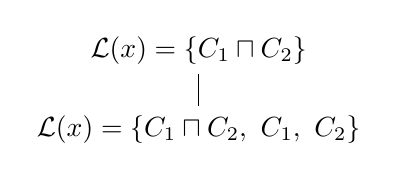
\begin{tikzpicture}[every text node part/.style={align=center},level 1/.style={level distance=1cm, sibling distance=3cm}]
\node [sibling distance=12cm] {$\mathcal{L}(x)=\{C_1\sqcap C_2\}$}
child { node []{$\mathcal{L}(x)=\{C_1\sqcap C_2,~C_1,~C_2\}$}
};
\end{tikzpicture} 
\end{center}
\item[$\sqcup$-rule:] if $C_1\sqcup C_2\in \mathcal{L}(x)$ and $\{C_1,C_2\} \cap \mathcal{L}(x)\neq \emptyset$, then $ \mathcal{L}(x)\rightarrow 
\mathcal{L}(x)\cup \{C\}~for ~some ~C\in\{C_1,C_2\}$.
\begin{center}
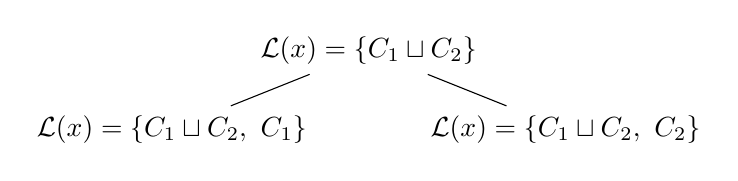
\begin{tikzpicture}[every text node part/.style={align=center},level 1/.style={level distance=1cm, sibling distance=5cm}]
\node [sibling distance=18cm] {$\mathcal{L}(x)=\{C_1\sqcup C_2\}$}
	      child{ node {$\mathcal{L}(x)=\{C_1\sqcup C_2,~C_1\}$}}
	      child{ node {$\mathcal{L}(x)=\{C_1\sqcup C_2,~C_2\}$}};
\end{tikzpicture} 
\end{center}
\item[$\exists$-rule:]  if $\exists r.C\in \mathcal{L}(x)$ and there does not exist a $y$ such that $\mathcal{E}(\langle x,y \rangle)$ and $C\in \mathcal{L}(y)$, then create a new node $y$ 
with $\mathcal{E}(\langle x,y\rangle)$ and $\mathcal{L}(y)=\{C\}$.
\begin{center}
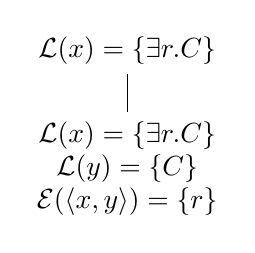
\begin{tikzpicture}[every text node part/.style={align=center},level 1/.style={level distance=1.5cm, sibling distance=3cm}]
\node [sibling distance=12cm] {$\mathcal{L}(x)=\{\exists r.C\}$}
child { node []{$\mathcal{L}(x)=\{\exists r.C\}$ \\ $\mathcal{L}(y)=\{C\}$ \\ $\mathcal{E}(\langle x,y \rangle)=\{r\}$}
};
\end{tikzpicture} 
\end{center}
\item[$\forall$-rule:] if $\forall r.C\in \mathcal{L}(x)$ and there exists a $y$ such that $\mathcal{E}(\langle x,y \rangle)$ and $C\notin \mathcal{L}(y)$,
then $ \mathcal{L}(y)\rightarrow  \mathcal{L}(y)\cup \{C\}$.
\begin{center}
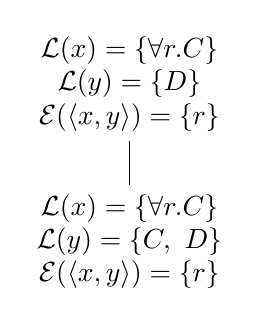
\begin{tikzpicture}[every text node part/.style={align=center},level 1/.style={level distance=2cm, sibling distance=3cm}]
\node [sibling distance=12cm] {$\mathcal{L}(x)=\{\forall r.C\}$\\ $\mathcal{L}(y)=\{D\}$ \\ $\mathcal{E}(\langle x,y \rangle)=\{r\}$}
child { node []{$\mathcal{L}(x)=\{\forall r.C\}$ \\ $\mathcal{L}(y)=\{C, ~D\}$ \\ $\mathcal{E}(\langle x,y \rangle)=\{r\}$}
};
\end{tikzpicture} 
\end{center}
\end{itemize}

\begin{mydef}(Clash)
A branch contains a clash if (i.e. the branch is closed), when $\{C,\neg C\}\subseteq \mathcal{L}(x)$ for a node $x$ and a concept $C$.
\end{mydef}
\begin{center}
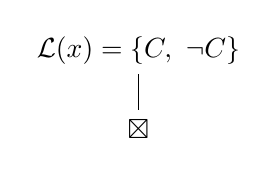
\begin{tikzpicture}[every text node part/.style={align=center},level 1/.style={level distance=1cm, sibling distance=3cm}]
\node [sibling distance=12cm] {$\mathcal{L}(x)=\{C,~\neg C \}$}
child { node []{$\boxtimes$}
};
\end{tikzpicture} 
\end{center}

A branch is said to be complete  when there exists a clash in some node $x$ or none of the rules mentioned above can be applied in the tableau. 
For a given concept $D$, $D ~ is ~ satisfiable$ if all the branches in the tableau are complete and at least one branch is open,
otherwise   $D ~ is ~ unsatisfiable$.



\section{Qualitative spatial reasoning}\label{sec:qsr}
Qualitative spatial relations have been studied from different views:
 topological relations (e.g. ``contains"), directional relative relations (e.g. ``left of" ), distances (e.g. ``close to") 
 as well as more complex relations (e.g. ``between")~\cite{Bloch2005fuzzy,freeman1975modelling,Hudelot2008fuzzy,kuipers1978modeling}. 
These relations are frequently used at a linguistic level by humans when describing a scene \cite{freksa1991qualitative}.
Even though quantitative information could be more precise, humans cannot use it as accurately as a machine.
Therefore, how to present qualitative information of human knowledge within the machine is a crucial research area in knowledge representation and reasoning.
The aim of our study is to apply human knowledge to the description of qualitative relationships and the reasoning tasks with spatial objects in a complex scene.
In this thesis, we consider some topological relations (inclusion and adjacency), direction and distance for spatial representation in a 3D space.
Qualitative spatial reasoning deals with the following questions, among others:
 \begin{itemize}
  \item Can we recognize an object from known objects and their spatial relations?
  \item Which relationships are satisfied between two objects when their relationships are not explicitly described in a given  knowledge base?
  \item Is a recognized spatial arrangement of a scene consistent with the given knowledge of the scene?
 \end{itemize}
 
 The reasoning tasks can be summarized as follows:
 \begin{enumerate}
  \item Determining whether an object satisfies a spatial configuration, where an object is described by an observation of spatial arrangement and 
  a spatial configuration is defined using expert knowledge. Then the task is considered as a consistency checking  of the observed object with respect to the spatial configuration in 
  the knowledge base.
  \item Determining the relationship between two objects from other spatial arrangements. The implicit relations between two objects can be inferred by other known spatial relations
  in a spatial arrangement.
  \item Determining the consistency of a spatial arrangement in a given configuration of the scene with respect to a specific domain knowledge. This task verifies the consistency
  between the observation and the spatial configuration defined using expert knowledge.
 \end{enumerate}

 In this section, we discuss different representations of spatial relations and illustrate our formalism to perform spatial reasoning.

\subsection{State of the art}
Chen \textit{et al.} discussed a broad range of spatial relation representations~\cite{chen2013survey}. Different spatial calculi are summarized for various aspects of space 
(topology, direction, distance, object shape, etc.). Basic qualitative spatial relations are summarized in Table~\ref{tab:sr}.
\begin{center}
\begin{table}[h]
   \begin{tabular}{| l | c | c |}
    \hline
    Topological relations~\cite{randell1992spatial} & Directional relations & Distance relations \\ \hline
    dc (``disconnected from'') & left of & far from \\ 
    eq (``equal with'', ``identical'') & right of & close to \\
    po (``intersect with'', ``partially overlaps'') & above  &   \\
    ec (``external connected with'',``touches'', ``adjacent'') & below &  \\
    tpp (``tangential proper part of'') & in front of &  \\
    tppi (``inversion of tpp'') &  behind  &   \\
    ntpp (``not tangential proper part of'') &   &  \\
    ntppi (``inversion of ntpp'') &  &  \\
    \hline
  \end{tabular}
  \caption{Basic spatial relations.}
  \label{tab:sr}  
\end{table}
\end{center}
\subsubsection{Topology}
Topology has been intensively investigated in qualitative spatial representation and the most popular representation is based on \textit{Region Connection Calculus} (RCC)~\cite{cohn1997qualitative}.
The collection $\{dc,~eq,~po,~ec,~tpp,~tppi,~ntpp,~ntppi\}$ is a set of disjoint exhaustive topological relations defined as RCC8~\cite{randell1992spatial}.
Between any two objects in topological space, only one of eight relations can hold.
Therefore, a useful reasoning mechanism of RCC8 based on a composition table is proposed in~\cite{egenhofer1991reasoning} (Table~\ref{tab:comptable}).
Let $A,B,C$ be three objects in a topological space, both $A,B$ and $B,C$ are adjacent ($ec$). Then the possible relations between $A,C$ can be found within the table.
This reasoning mechanism allows answering the second and third questions of qualitative spatial reasoning problems. 
However, the composition table only gives possible relations and many of composition rules give no information like $dc(A,B)$ and $dc(B,C)$ (all the relations possibly
hold between $A$ and $C$ from the composition table).
Furthermore, the RCC8 representation and composition table were constructed for determining a satisfaction problem 
in a specific arrangement~\cite{wessel2000obstacle,wessel00alcra}.
Unfortunately, the inference within this kind of representation is undecidable~\cite{wessel2000obstacle}. 
Lutz \textit{et al.} exploited qualitative reasoning in concrete domains with constraint satisfaction problems~\cite{lutz2007tableau}.
The authors described a constraints network in the concrete domain based on RCC8 relations. The spatial reasoning is 
tackled by checking existence of an appropriate network in the concrete domain.
In the context of brain anatomy, only the inclusion relations are included in the work in~\cite{santos2012region}.
Therefore, inclusion relations and adjacency, considered in this thesis, are frequently used in the spatial knowledge of the  brain anatomy. 
The property of transitivity  is emphasized in this context. 
 \begin{center}
 \begin{table}[H]
    \begin{tabular}{|p{1cm} || p{1.5cm} | p{1.5cm} | p{1.5cm} | p{1.5cm} | p{1.5cm} |p{1.5cm} |p{1.5cm}| p{1.5cm}| }
    \hline
      & $dc$ (B,C) & $\textbf{ec}$ $\textbf{(B,C)}$ & $eq$ (B,C) & $ntpp$  (B,C) & $tpp$ (B,C) &  $ntppi$ (B,C) & $tppi$ (B,C)& $op$ (B,C)\\ \hhline{|=|=|=|=|=|=|=|=|=|}
    $dc$ (A,B) & $dc$ or $ec$ or $eq$ or $ntpp$ or $tpp$ or $ntppi$ or $tppi$ or $op$  & $dc$ or $ec$ or $ntpp$ or $tpp$ or $op$ & $dc$ & $dc$ or $ec$ or $ntpp$ or $tpp$ or $op$ 
		& $dc$ or $ec$ or $ntpp$ or $tpp$ or $op$ & $dc$ &  $dc$ & $dc$ or $ec$ or $ntpp$ or $tpp$ or $op$ \\ \hline 
    $\textbf{ec}$ $\textbf{(A,B)}$ & $dc$ or $ec$ or $eq$ or $ntpp$ or $tpp$ or $ntppi$ or $tppi$ or $op$  & $\textbf{dc~or ec}$ $\textbf{or ntpp}$ $\textbf{or tpp}$ $\textbf{or op}$ & $dc$ 
    & $dc$ or $ec$ or $ntpp$ or $tpp$ or $op$ 	& $dc$ or $ec$ or $ntpp$ or $tpp$ or $op$ & $dc$ &  $dc$ & $dc$ or $ec$ or $ntpp$ or $tpp$ or $op$ \\ \hline 
    $eq$  (A,B) & $dc$ & $ec$ & $eq$ & $ntpp$ & $tpp$ & $ntppi$ & $tppi$ & $op$\\ \hline
    $ntpp$  (A,B)& $dc$ & $dc$ & $ntpp$ & $ntpp$ & $ntpp$ & $dc$ or $ec$ or $eq$ or $ntpp$ or $tpp$ or $ntppi$ or $tppi$ or $op$  & 
		  $dc$ or $ec$ or  $ntpp$ or $tpp$ or $op$& $dc$ or $ec$ or  $ntpp$ or $tpp$ or $op$\\ \hline
    $tpp$  (A,B)& $dc$ & $dc$ or $ec$  & $tpp$ & $ntpp$ & $tpp$ or $ntpp$ & $dc$ or $ec$ or $ntppi$ or $tppi$ or $op$ & $dc$ or $ec$ or $eq$ or $tpp$ or $tppi$ or $op$ &
		   $dc$ or $ec$ or $ntpp$ or $tpp$ or $op$ \\ \hline
    $ntppi$ (A,B)& $dc$ or $ec$ or $ntppi$ or $tppi$ or $op$ & $ntppi$ or $tppi$ or $op$  & $ntppi$ & $eq$ or $ntpp$ or $tpp$ or $tppi$ or $ntppi$ or $op$ &$tppi$ or $ntppi$ or $op$
		  & $ntppi$ &$ntppi$ & $tppi$ or $ntppi$ or $op$ \\ \hline
    $tppi$ (A,B)& $dc$ or $ec$ or $ntppi$ or $tppi$ or $op$  & $ec$ or $ntppi$ or $tppi$ or $op$ & $tppi$ & $ntpp$ or $tpp$ or $op$ & $eq$ or $tpp$ or $tppi$ or $op$ & $ntppi$  &
		  $ntppi$ or $tppi$ & $ntppi$ or $tppi$ or $op$\\ \hline
    $op$ (A,B)& $dc$ or $ec$ or $ntppi$ or $tppi$ or $op$ & $dc$ or $ec$ or $ntppi$ or $tppi$ or $op$ & $op$ & $ntpp$ or $tpp$ or $op$ & $ntpp$ or $tpp$ or $op$ &
		  $dc$ or $ec$ or $ntppi$ or $tppi$ or $op$  & $dc$ or $ec$ or $ntppi$ or $tppi$ or $op$ & $dc$ or $ec$ or $eq$ or $ntpp$ or $tpp$ or $ntppi$ or $tppi$ or $op$\\ \hline
    \end{tabular}
    \caption{The 64 compositions of binary topological relations between objects $A$ and $C$ via the third object $B$. Extracted from~\cite{egenhofer1991reasoning}.}
    \label{tab:comptable}
\end{table}
\end{center} 
\subsubsection{Direction}
Directional relations are seen as primarily important spatial relationships in brain anatomical images~\cite{Bloch2005fuzzy,fouquier2012sequential,Hudelot2008fuzzy,nempont2013constraint}.
As mentioned in~\cite{Bloch2005fuzzy}, a direction is defined by a \textit{target object}, a \textit{reference object} and a \textit{reference system}.
In an 3D space, directional relations are represented by six basic terms (e.g. right, above, behind, etc.).
In order to compute directional relationships between two objects, many methods such as histograms of angles and morphological approaches are summarized in~\cite{Bloch2005fuzzy}.
A fuzzy representation is employed in these approaches. 
For instance, a fuzzy set (fuzzy landscape) representing the region of space where a given directional relation with respect to a reference object is satisfied 
can be computed using a morphological dilation with an appropriate structuring element of the reference object.
The satisfaction degree of the direction between the target object and the reference object is evaluated by comparison between the target object and the fuzzy landscape.
In a crisp setting, two strategy are usually employed: point based and extend object based (bounding box)~\cite{chen2013survey}.
However, both of the two representations ignore the influence of object shape. The representation is not as accurate to human intuition as a fuzzy representation.
\subsubsection{Distance}
Qualitative representation of the distance between two objects depends on the metric measures about the geometrical information of the specific domain.
The measure is often calculated in terms of Euclidean distance, considering two objects as two points. In a complex scene, which the shape cannot be ignored,
distance can benefit from minimum distance, mean distance and Hausdorff distance, etc.~\cite{Bloch2005fuzzy}. One useful scale system to convert numerical measures into 
qualitative representations uses fuzzy sets for defining satisfaction degrees of different qualitative representations~\cite{Bloch2005fuzzy}.

\subsection{Qualitative spatial reasoning in $\mathcal{ALCHI_{R^+}}$}
In this section, we give the logical formalism to represent qualitative spatial relationships as roles and  corresponding properties in terms of role axioms within a role box.
Then, we illustrate how the qualitative spatial reasoning is developed using this logical formalism. 
\subsubsection{Syntax and semantics of roles}
\begin{mydef}(Role syntax)
 Let $N_R$ be  a set of role names, the inverse roles and the negation of roles are represented by $r^-$ and $\neg r$.
 Complex roles are characterized with $r_1\sqcap r_2$ and $r_1\sqcup r_2$.
 Role axioms are used for modeling properties of roles such as inclusion ($r_1\sqsubseteq r_2$) and role composition ($r_1 \circ r_2$).
\end{mydef}
Table \ref{tab:synrole} describes a main syntax and semantics of roles for Description Logics.
\begin{center}
\begin{table}[h]
   \begin{tabular}{| l | c | r |}
    \hline
    Constructor & Syntax & Semantics \\ \hline
    Atomic role & $r$ & $r^\mathcal{I}\subseteq \Delta^\mathcal{I} \times \Delta^\mathcal{I}$ \\
    Inverse role & $r^-$ & $\{\langle x,y\rangle,~x\in \Delta^\mathcal{I},~y\in \Delta^\mathcal{I} | ~\langle y,x \rangle\in r^\mathcal{I}\}$ \\ 
    Role negation & $\neg r$ & $\Delta^\mathcal{I} \times \Delta^\mathcal{I} \setminus r^\mathcal{I}$ \\
    Role composition & $r_1\circ r_2$ & $\{\langle x,z\rangle, x\in \Delta^\mathcal{I},~z\in \Delta^\mathcal{I}| \exists y\in \Delta^\mathcal{I}, 
\langle x,y\rangle\in r_1^\mathcal{I}~and~\langle y,z\rangle\in r_2^\mathcal{I}\}$  \\
    Role conjunction & $r_1\sqcap r_2$ & $r_1^\mathcal{I} \cap r_2^\mathcal{I}$ \\
    Role disjunction & $r_1\sqcup r_2$ & $r_1^\mathcal{I} \cup r_2^\mathcal{I}$ \\
    Role inclusion & $r_1\sqsubseteq r_2$ &  $r_1^\mathcal{I} \subseteq r_2^\mathcal{I}$\\
    Role equivalence & $r_1\equiv r_2$ & $r_1^\mathcal{I} = r_2^\mathcal{I}$\\
    \hline
  \end{tabular}
  \caption{Basic role relations.}
  \label{tab:synrole}  
\end{table}
\end{center}

\begin{mydef}(Role inclusion axiom) 
 A role inclusion axiom is defined in the form:
 $$r\sqsubseteq s,$$
 where $r$ and $s$ are basic roles in $N_R$ or complex roles built with role constructors. A role equivalence $r\equiv s$ can be rewritten in the form $r\sqsubseteq s$ and $s\sqsubseteq r$.
\end{mydef}
\begin{mydef}(RBox)
A role box, denoted by RBox, is a finite set
of axioms for $N_R$  based on a set of roles $\mathbf{R}=N_R\cup\{r^-| r\in N_R\}$, where $r^-$  represents the inversion of role $r$.
Based on role inclusion and role equivalence, role axioms characterize role properties as follows:
\begin{itemize}
 \item role composition: $u\circ v \sqsubseteq r_1\sqcup \cdots\sqcup r_n$ with $n\geqslant 1$, which is interpreted as 
 $(u\circ v)^\mathcal{I} \subseteq r_1^\mathcal{I} \cup \cdots \cup r_n^\mathcal{I}$. For all three interpretation elements $x,y,z\in \Delta^\mathcal{I}$, 
 ($\langle x,y \rangle \in u^\mathcal{I}$ and $\langle y,z \rangle \in v^\mathcal{I}$) implies  $\langle x,z \rangle \in r_1^\mathcal{I} \cup \cdots \cup r_n^\mathcal{I}$. 
 \item transitive role: $r\circ r \sqsubseteq r$, which is interpreted as $(r\circ r)^\mathcal{I} \subseteq r^\mathcal{I}$. If there exist three interpretation elements
 $x,y,z\in \Delta^\mathcal{I}$, $\langle x,y \rangle \in r^\mathcal{I}$ and $\langle y,z \rangle \in r^\mathcal{I}$ implies  $\langle x,z \rangle \in r^\mathcal{I}$.
 \item inverse roles: $u \equiv v^-$, which is interpreted as $u^\mathcal{I} = v^{-\mathcal{I}}$. For all two interpretation elements  $x,y\in \Delta^\mathcal{I}$,
 then $\langle x,y \rangle \in u^\mathcal{I}$ iff $\langle y,x \rangle \in v^\mathcal{I}$.
 \item symmetric role: $r \equiv r^-$, which is interpreted as $r^\mathcal{I} = r^{-\mathcal{I}}$. For all two interpretation elements  $x,y\in \Delta^\mathcal{I}$,
 then $\langle x,y \rangle \in r^\mathcal{I}$ iff $\langle y,x \rangle \in r^\mathcal{I}$.
 \item disjoint roles: $u\sqsubseteq \neg v$. which is interpreted as $u^\mathcal{I} \subseteq \Delta^\mathcal{I} \setminus v^\mathcal{I}$ or $u^\mathcal{I}\cap v^\mathcal{I}=\emptyset$. 
 For all two interpretation elements  $x,y\in \Delta^\mathcal{I}$, 
$\langle x,y \rangle \in u^\mathcal{I}$ implies $\langle x,y \rangle \notin v^\mathcal{I}$.
\end{itemize}
\end{mydef}
The knowledge base used for spatial reasoning in our framework is built with three blocks: terminologies (TBox), role axioms (RBox) and assertions (ABox)
($\mathcal{K}=\{\mathcal{T},\mathcal{R},\mathcal{A}\}$).

A decidable DL language $\mathcal{ALCHI_{R_+}}$~\cite{horrocks1999description} is described in the following for the qualitative spatial reasoning, where the spatial relations are 
represented by roles and the properties of these spatial relations can be represented by the axioms in the RBox.

The table of syntax and semantics of $\mathcal{ALCHI_{R_+}}$ is shown as follows:
 \begin{center}
 \begin{table}[H]
    \begin{tabular}{|p{4cm} | p{2cm} | p{10cm}| }
    \hline
      Name & Syntax & Semantics \\ \hline
    Top & $\top$ & $\Delta^\mathcal{I}$ \\
    Bottom & $\bot$ & $\emptyset$ \\ 
    Negation & $\neg C$ & $\Delta^\mathcal{I}\setminus C^\mathcal{I}$ \\ 
    Conjunction & $C\sqcap D$ & $C^\mathcal{I}\cap D^\mathcal{I}$  \\  
    Disjunction & $C\sqcup D$ &  $C^\mathcal{I}\cup D^\mathcal{I}$ \\  
    Existential restriction & $\exists r.C$ & $\{x\in \Delta^\mathcal{I}~|~ \exists y\in \Delta^\mathcal{I}, \langle x,y\rangle \in r^\mathcal{I}~and~y\in C^\mathcal{I}\}$ \\ 
    Universal restriction & $\forall r.C$ & $\{x\in \Delta^\mathcal{I}~|~ \forall~y\in \Delta^\mathcal{I}, \langle x,y\rangle \in r^\mathcal{I}~implies~y\in C^\mathcal{I}\}$ \\ \hline
    Atomic role & $r$ & $r^\mathcal{I}\subseteq \Delta^\mathcal{I} \times \Delta^\mathcal{I}$\\
    Inverse role & $r^-$ & $\{\langle x,y \rangle,~x\in \Delta^\mathcal{I},~y\in \Delta^\mathcal{I} | ~\langle y,x \rangle\in r^\mathcal{I}\}$\\ 
    Role composition & $r_1\circ r_2$ & $\{\langle x,z\rangle, x\in \Delta^\mathcal{I},~z\in \Delta^\mathcal{I}| \exists y\in \Delta^\mathcal{I},\langle x,y \rangle\in r_1^\mathcal{I}~and~\langle y,z\rangle\in r_2^\mathcal{I}\}$\\
    Role conjunction & $r_1\sqcap r_2$ & $r_1^\mathcal{I} \cap r_2^\mathcal{I}$ \\
    Role disjunction & $r_1\sqcup r_2$ & $r_1^\mathcal{I} \cup r_2^\mathcal{I}$ \\
    Role inclusion & $r_1\sqsubseteq r_2$ &  $r_1^\mathcal{I} \subseteq r_2^\mathcal{I}$\\
    Role equivalence & $r_1\equiv r_2$ & $r_1^\mathcal{I} = r_2^\mathcal{I}$\\    \hline
    Subsumption & $C\sqsubseteq D$ & $C^\mathcal{I}\subseteq D^\mathcal{I}$ for all $\mathcal{I}$\\
    Concept Definition & $C\equiv D$ & $C^\mathcal{I}= D^\mathcal{I}$ for all $\mathcal{I}$\\ \hline
    Concept assertion & $a:C$ & $a^\mathcal{I}\in C^\mathcal{I}$ \\
    Role assertion & $(a,b):r$ & $(a^\mathcal{I},b^\mathcal{I})\in r^\mathcal{I}$ \\ \hline
    \end{tabular}
    \caption{Syntax and semantics of $\mathcal{ALCHI_{R_+}}$.}
    \label{tab:interpretation}
\end{table}
\end{center} 
We elaborate on Definition~\ref{def:tableauALC} for an $\mathcal{ALCHI_{R+}}$ tableau by adding new properties and associated rules as follows.
\begin{enumerate}
\setcounter{enumi}{5}
\item if $\forall r.C\in \mathcal{L}(x)$ and $r$ is a transitive role, then for all $y \in \mathbf{S}$ such that $r \in \mathcal{E}(\langle x,y\rangle)$, 
$\forall r.C\in\mathcal{L}(y)$.

$\forall r_{trans}$-rule: if $\forall r.C\in \mathcal{L}(x)$ which $r$ is transitive and there exists a $y$ such that $\mathcal{E}(\langle x,y \rangle)$,
then $ \mathcal{L}(y)\rightarrow  \mathcal{L}(y)\cup \{\forall r.C\}$.
\begin{center}
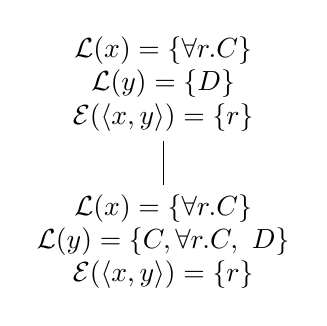
\begin{tikzpicture}[every text node part/.style={align=center},level 1/.style={level distance=2cm, sibling distance=3cm}]
\node [sibling distance=12cm] {$\mathcal{L}(x)=\{\forall r.C\}$\\ $\mathcal{L}(y)=\{D\}$ \\ $\mathcal{E}(\langle x,y \rangle)=\{r\}$}
child { node []{$\mathcal{L}(x)=\{\forall r.C\}$ \\ $\mathcal{L}(y)=\{C,\forall r.C, ~D\}$ \\ $\mathcal{E}(\langle x,y \rangle)=\{r\}$}
};
\end{tikzpicture} 
\end{center}
\item $r \in \mathcal{E}(\langle x,y\rangle)$ iff  $ r^-\in \mathcal{E}(\langle y,x\rangle)$.

$r^-$-rule: if $r\in\mathcal{E}(\langle x,y \rangle)$,
then $r^-\in\mathcal{E}(\langle y,x \rangle)$.
\begin{center}
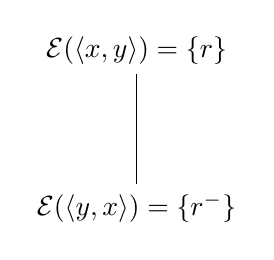
\begin{tikzpicture}[every text node part/.style={align=center},level 1/.style={level distance=2cm, sibling distance=3cm}]
\node [sibling distance=12cm] {$\mathcal{E}(\langle x,y \rangle)=\{r\}$}
child { node []{$\mathcal{E}(\langle y,x \rangle)=\{r^-\}$}
};
\end{tikzpicture} 
\end{center}

\item if $ r\in \mathcal{E}(\langle x,y\rangle)$ and $r\sqsubseteq v$ (or $r^-\sqsubseteq v^-$) then  $v \in \mathcal{E}(\langle x,y\rangle)$.

$r_\sqsubseteq$-rule
\begin{center}
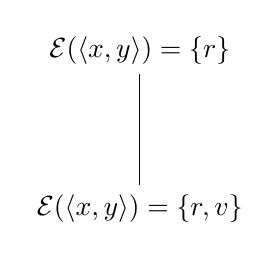
\begin{tikzpicture}[every text node part/.style={align=center},level 1/.style={level distance=2cm, sibling distance=3cm}]
\node [sibling distance=12cm] {$\mathcal{E}(\langle x,y \rangle)=\{r\}$}
child { node []{$\mathcal{E}(\langle x,y \rangle)=\{r,v\}$}
};
\end{tikzpicture} 
\end{center}
\end{enumerate}

\subsection{From image to symbolic representation}
 This section deals with the computation of qualitative relationships in a segmented image and the construction of a symbolic representation for the observation. 
The transformation of representation space from low-level numerical data to symbolic level is the first phase of the framework.
Concretely, objects and spatial information are extracted and represented within terminologies using an ABox.
Furthermore, the symbolic representation can be used for  reasoning service in the logical formalism.

\begin{figure}[h]
 \centering
 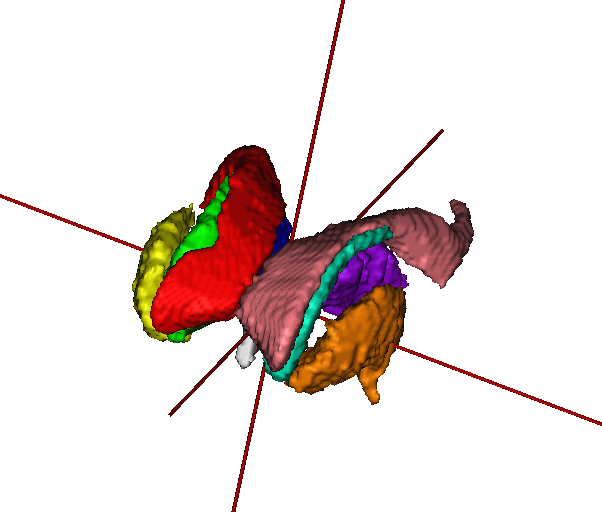
\includegraphics[width=.3\textwidth]{./figures/mesh_all_vue_45.png}
 \caption{\label{fig:brain3d}A segmented brain volume (structures are marked by different colors, e.g. the left lateral ventricle is in red.).}
\end{figure}
As  shown in Figure \ref{fig:brain3d}, spatial relationships between structures in brain is an important feature for the image interpretation. 
Here we consider directional relations, computed using angle histograms.
The satisfaction degree for a given direction is computed as the intersection of the histogram and the fuzzy set defining the semantics of direction (Figure~\ref{fig:right}).

We take the right caudate nucleus (target object) and the right lateral ventricle (reference object)\footnote{Here we use ``right'' to represent 
structures in the right part of image for the simplicity of visualization (i.e. the structure in the right part of image is the left part in the brain.)} as an example to illustrate the computation.
The structures are presented in Figure \ref{fig:sturctpair}.
The histogram of angles includes the count of angles of each pair of voxels in the right caudate nucleus and the right lateral ventricle.
The angle is composed by a pair $\alpha_1$ and $\alpha_2$. 
$\alpha_1$ takes value in $[-\pi, \pi]$ by measuring the angle between the projection of the segment joining two voxels on the x-y coordinate plane and the x-coordinate axis.
$\alpha_2$ measures the angle between the segment and the x-y projection, and takes value in $[-\pi/2, \pi/2]$.
The histogram is normalized and contains 256 bins for $\alpha_1$ and 128 bins for $\alpha_2$ as shown in Figure \ref{fig:histopair}.
For each two pair of structures, six satisfaction degrees can be computed for each direction (i.e. ``right'', ``left'', ``above'', ``below'', ``in front of'', ``behind''.).


\begin{figure}[h]
 \centering
 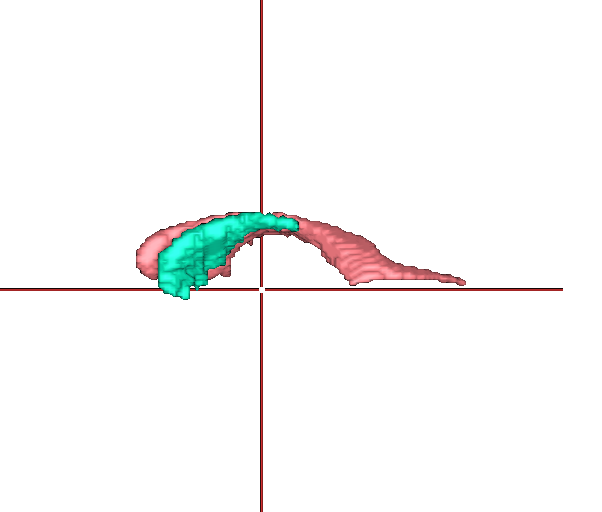
\includegraphics[width=.3\textwidth]{./figures/right_lvl_cdl.png}
 \caption{\label{fig:sturctpair}The right lateral ventricle and the right caudate nucleus seen from the right side.}
\end{figure}
% qualitative spatial relation is evaluated by computing histogram of angles between two objects and comparison with fuzzy set of a certain direction.
\begin{figure}[h]
 \centering
 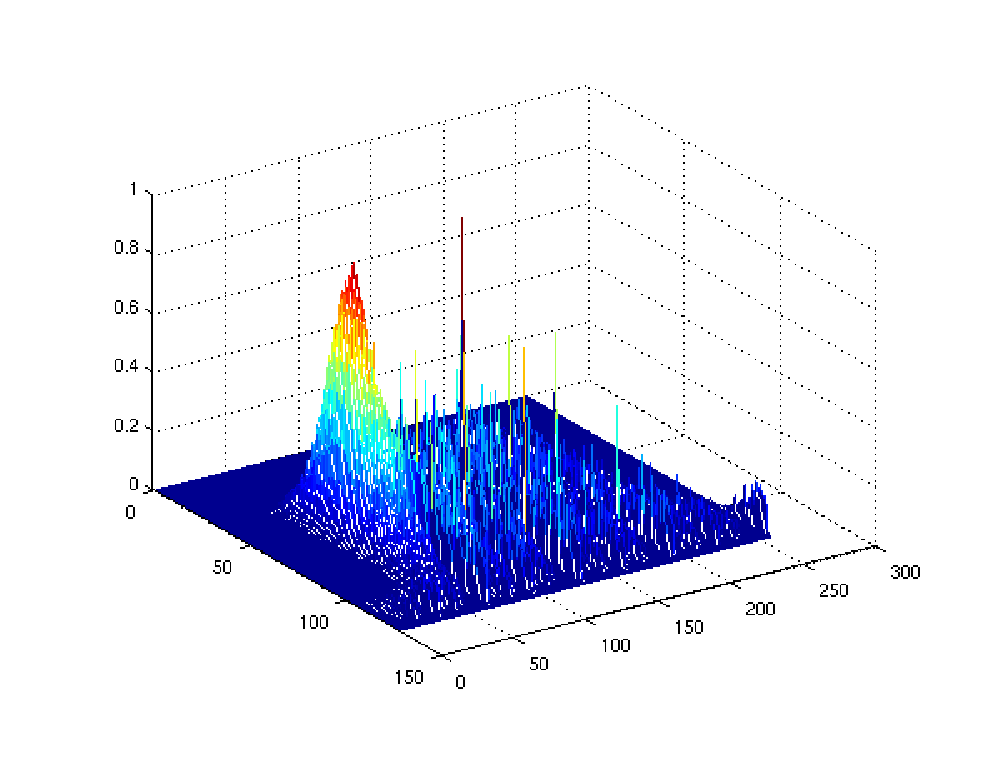
\includegraphics[width=.5\textwidth]{./figures/right_cdl_lvl_crop.pdf}
 \caption{\label{fig:histopair}The histogram of angles between right lateral ventricle and right caudate nucleus.}
\end{figure}

\begin{figure}[h]
 \centering
 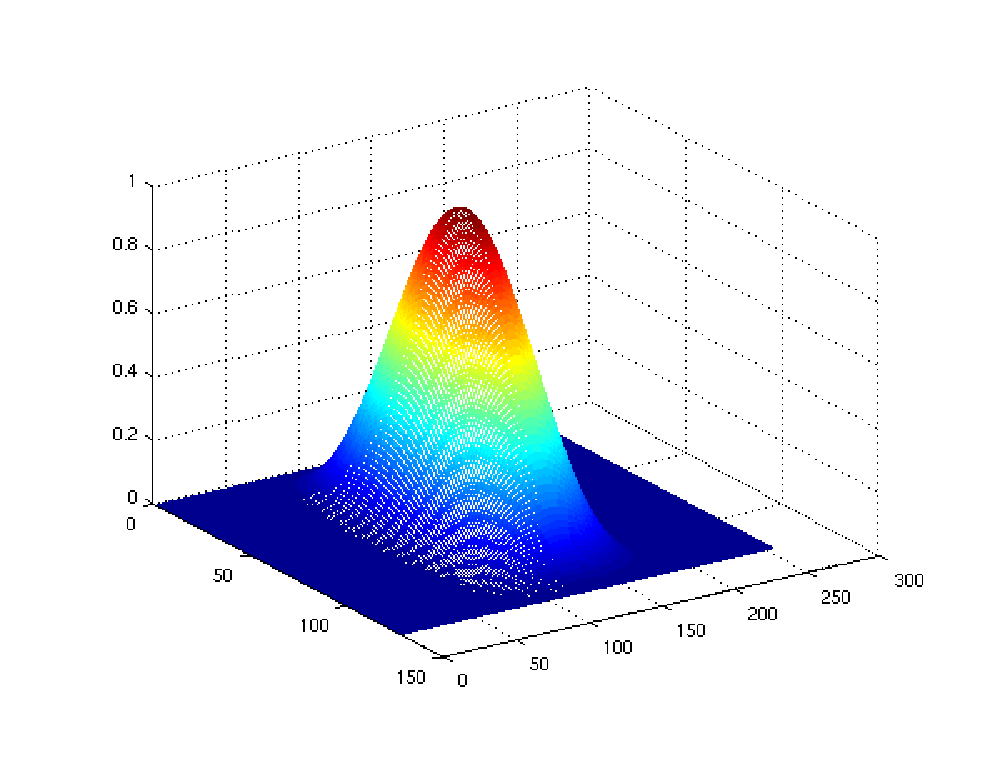
\includegraphics[width=.5\textwidth]{./figures/right_crop.pdf}
 \caption{\label{fig:right}Fuzzy relation ``right''.}
\end{figure}

\begin{figure}[h]
 \centering
 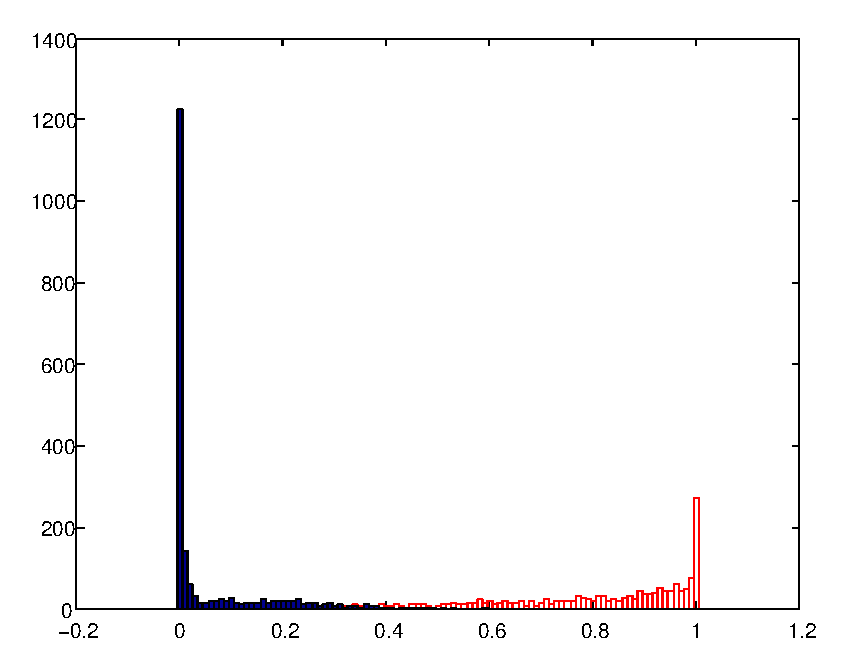
\includegraphics[width=.5\textwidth]{./figures/right_nright_thresh_crop.pdf}
 \caption{\label{fig:thresh}The histogram of intersection degree of the satisfied pairs (red bins) and the ones of the other part. The vertical line indicates the optimized threshold value.}
\end{figure}

Then we demonstrate how to choose a threshold in order to convert fuzzy relations to crisp ones and to use these relations in our logical framework.
For choosing a threshold $t$ for every direction, we manually select all the pairs of structures which satisfy the relation and all the unsatisfied pairs.
We take the histogram of intersection degrees of the satisfied pairs (red bins) and the ones of the other part (blue bins) (Figure \ref{fig:thresh}).
Then the threshold is taken by minimizing the error of mis-classification:
$E=\frac{\sharp(x_1>threshold)}{\sharp(x_1)}+\frac{\sharp(x_2<threshold)}{\sharp(x_2)}$ where $x_1$ (resp. $x_2$) represents unsatisfied pairs (resp. satisfied pairs) 
and $\sharp(x_1>threshold)$ (resp. $\sharp(x_2>threshold)$) represents the number of mis-classification of unsatisfied pairs (resp. the number of mis-classification of satisfied pairs).

The symbolic representation is generated in an ABox. All the detected structures and spatial relations are saved in a structural XML file using corresponding alias.
A simple example is given in Figure \ref{fig:owlfile}.
\begin{figure}[h]
 \centering
 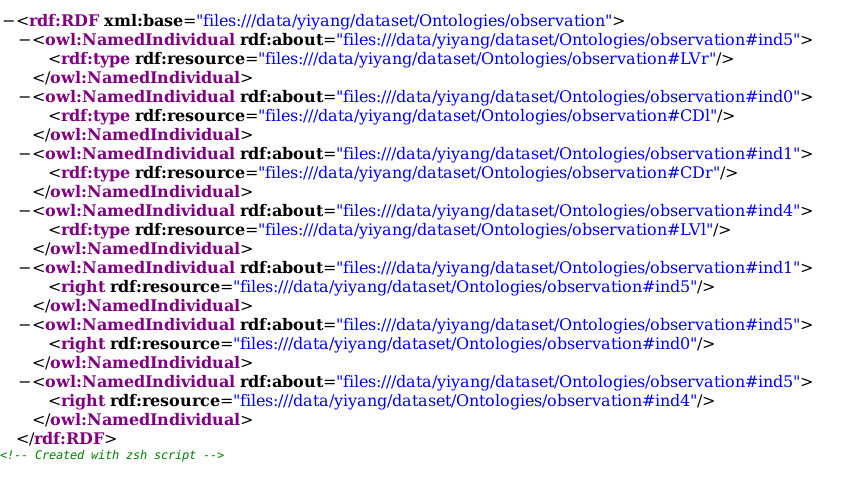
\includegraphics[width=.8\textwidth]{./figures/xml_screenshot.png}
 \caption{\label{fig:owlfile}A sample of the ABox.}
\end{figure}

\subsection{Example}
 The complete knowledge base is given as follows:
\begin{align*}
 TBox=\{ Hemisphere &\sqsubseteq \exists isPartOf. Brain\\
	 BrainStructure &\sqsubseteq \exists isPartOf. Brain\\
	 BrainDisease &\sqsubseteq \exists isPartOf. Brain \sqcap \neg BrainStructure\\
	 Tumor  &\sqsubseteq BrainDisease\\
	 LVl &\sqsubseteq BrainStructure \sqcap \exists (rightOf \sqcap closeTo). CNl\\
	 LVr &\sqsubseteq BrainStructure \sqcap \exists (leftOf \sqcap closeTo). CNr\\
	 CNl &\sqsubseteq BrainStructure\\
	 CNr &\sqsubseteq BrainStructure\}
\end{align*}
The role axioms are described as:
\begin{align*}
 RBox=\{ rightOf &\equiv leftOf^-\\
         above &\equiv below^- \\
	 closeTo &\equiv closeTo^- \\
	 farFrom &\equiv farFrom^- \\
	 isPartOf \circ isPartOf &\sqsubseteq isPartOf \\
	 hasPart \circ hasPart &\sqsubseteq hasPart\\
	 isPartOf &\equiv hasPart^-\}
\end{align*}
The ABox represents the observation of structures in an image and the relationships between them.
In this example, both recognized and unrecognized structures are represented by individuals. Spatial relations between the unknown structure ($b$) and
recognized structures ($a,c$) are represented by roles.
For instance, a region is recognized as the left caudate nucleus (CNl), denoted by $a$.
The region of brain is denoted by $c$. An unknown region is segmented and their relationships are computed.  
Such an observation can be represented as
\begin{align*}
 ABox=\{ a&: CNl \\
	 b&: Unknown~Object \\
	 c&: Brain \\
	 \langle a,b\rangle &: leftOf, closeTo \\
	 \langle b,c\rangle &: isPartOf\}
\end{align*}
In this example, the ABox describes an observation of a given scene and the objective is to find a reasonable description of  the unknown object $b$.
Therefore, the relationships between $b$ and other individuals are important for the reasoning. 
We demonstrate the spatial reasoning by a concept subsumption test using the tableau method in the Appendix A.
The subsumption test of the example in the appendix (which can be seen as an abductive reasoning) provides a tableau approach to answer the first question of the spatial reasoning
problem (recognition of an unknown object using the background knowledge and the spatial arrangements in the observation).
In the first step, we can derive $\langle b,a\rangle:leftOf^-,closeTo^-$ from $\langle a,b\rangle:leftOf,closeTo$ using the inverse property of roles.
By the definition $rightOf\equiv leftOf^-$ and $closeTo\equiv closeTo^-$ in RBox, the spatial relationship $rightOf,closeTo$ between $b$ and $a$ can be deducted.
Another type of spatial reasoning consists in verifying inclusion relations by using the transitive property of transitive roles like $isPartOf$ in tableau method. 
This type of reasoning answers the second question in a restricted way. For a transitive role (e.g. $isPartOf$), we can check the satisfiability of the relation
between two objects via the third one. The Rule 6 in the Section 3.2 provides a corresponding rule to verify the implicit transitive relation in tableau method. 
In the example, $\exists isPartOf. Hemisphere \sqsubseteq \exists isPartOf.Brain$ is verified.
This example is modeled as a test of satisfiability problem which can be seen as the answer for the third question.
These simple spatial reasonings are not as powerful as those in the references, however, we consider the objects as a set of pixels instead of approximating an object by a single pixel 
(the transitivity of direction does not hold any more).
In addition, topological relations and spatial reasoning on compositions are still an open problem.

\section{Abductive reasoning}\label{sec:abd}
Abductive reasoning is a backward-chaining inference, consisting in generating hypotheses and finding the ``best'' explanation of a given observation.
Unlike the standard reasoning presented in Section~\ref{sec:pre}, abductive reasoning is a non-monotonic reasoning because the conclusion is not necessarily correct.
New knowledge should be added in order to positively entail the observation.
Image interpretation can be expressed as an abductive reasoning  mechanism.
When facing a pathological brain image, an expert has to resort to his knowledge of pathological anatomy, in order to give  an explanation for the observed image. 
In this section, we will introduce how abduction is applied in image interpretation from two aspects (generation of hypotheses and selection of a preferred explanation).
\subsection{State of the art of abductive reasoning}
The term ``Abduction'' was first proposed by Charles S. Peirce in philosophy.
Afterwards, abduction has been developed in artificial intelligence and cognitive science.
Aliseda~\cite{aliseda1997seeking} gave a general overview of abduction in propositional logic and proposed tableaux methods for abduction.
In the context of Description Logics, four types of abduction problems  are described by Elsenbroich~\cite{elsenbroich2006case}.
Let $\mathcal{L}$ be a DL, $\mathcal{K}=\{\mathcal{T},\mathcal{A}\}$ be a knowledge base in $\mathcal{L}$, $C,D$ two concepts in $\mathcal{L}$ and suppose that they are satisfiable
with respect to  $\mathcal{K}$.
The logical formalisms of abduction in DLs are represented as follows:
\begin{itemize}
 \item Concept abduction: given an observation concept $O$, a hypothesis is a concept $H$ such that $\mathcal{K}\vDash H \sqsubseteq O$.
 \item TBox abduction: let $C\sqsubseteq D$ be satisfiable w.r.t $\mathcal{K}$, the hypothesis is a set of axioms $S_T=\{E_i\sqsubseteq F_i \mid i\leq n\}$
 such that $ \mathcal{K}\cup S_T\vDash C\sqsubseteq D$.
 \item ABox abduction: let $S_a$ be a set of assertions representing the observation, a hypothesis is a set $S_b$ of ABox assertions such that $\mathcal{K} \cup S_b\vDash S_a$.
 \item Knowledge base abduction: let $\phi$ be a consistent set of ABox or TBox assertions w.r.t. $\mathcal{K}$. A solution of knowledge base abduction, considered 
 as a combination of TBox abduction and ABox abduction, is any finite set $S=\{\psi_i \mid i\leq n\}$ such that $ \mathcal{K} \cup S \vDash \phi$.
\end{itemize}

An explanation $H$ for an abduction problem has the following properties: 
\begin{itemize}
  \item Consistency: $\mathcal{K}\cup H$ is consistent.
  \item Relevance: $\phi$ is not entailed by $H$ ($H\nvDash \phi$).
  \item Semantic minimality: there does not exist a hypothesis $H_i$ such that $H_i\vDash H$.
 \end{itemize}
Image interpretation task was regarded as an abduction problem in \cite{atif2014explanatory,gries2010probabilistic,neumann2008scene,shanahan2005perception}.
In \cite{neumann2008scene}, DL-safe rules were proposed to map high level concepts and occurrence objects in the scene and their relationships.
The rules ensure the expressivity and preserve the decidability of the reasoning. However, only the concept defined in the rules can be inferred using 
the formalism. In \cite{atif2014explanatory}, the image interpretation was formulated as a concept abduction problem.
The DL is expressed in $\mathcal{EL}$. The knowledge base is processed using formal concept analysis and the abductive reasoning is tackled
by a recursive erosion on the lattice based representation. In this way, not only defined concepts but also undefined complex concepts can be inferred.
% \cite{shanahan2005perception} multimedia interpretation as abduction.
% \cite{gries2010probabilistic}


% di2009tableaux
Apart from the abduction mechanism mentioned above, the tableau method is an effective approach for solving abduction problems.
The tableau method was first adapted in Description Logics formalisms for a market matchmaking problem~\cite{colucci2004uniform}.
Colucci \textit{et al.} modeled this problem as a concept abduction in the DL $\mathcal{ALN}$ \cite{colucci2004uniform},
where the observations are the demand and the supply is treated as the explanation for the meet of the request.
The tableau method has also been studied by Halland \textit{et al.} in \cite{halland2014tbox} for a TBox abduction problem.
For a TBox abduction problem, a TBox axiom in the form $\phi= C\sqsubseteq D$ is an explanation enforcing the entailment of the observation,
which is also in the form of  a TBox subsumption form. Similar to the tableau method for the  concept abduction, if the disjunction of
two concepts $A_1$  and $\neg A_2$ can create a clash of the tableau, then $A_2 \sqsubseteq A_1$ is considered as a potential explanation.


Klarman \textit{et al.}~\cite{klarman2011abox} present a tableau method for the ABox abduction in $\mathcal{ALC}$.
This method integrates logic reasoning techniques of the first-order logic. First, knowledge and observation are
transformed into first-order logic. Then, a tableau in the context of the first-order logic is built and solutions
are selected in the open branches. The results are transformed into Description Logic from the first-order logic in the end.
In \cite{du2011towards,du2014tractable}, the authors also focus on ABox abduction problems. 
In~\cite{du2014tractable}, Du \textit{et al.} introduced a tractable approach to ABox abduction, called the query abduction problem.
This problem focuses on giving the explanations, which are new facts neither in the observation nor in the assertional knowledge, for an observation.
The observation is represented by a Boolean conjunctive query in the form $\exists x\Phi(x,c)$, where $\Phi(x,c)$ is a conjunction of concepts
assertions and role assertions and $x$ represents a variable and $c$ represents an individual.
However, the potential hypotheses are restricted to atomic concepts and roles in the TBox.

We then move to the other aspect of abduction problem: the selection problem.
As a set of syntactical candidates generated using the tableau method, the selection relies on explicit restrictions for choosing the ``best'' explanation.
Restrictions concern filtering out inappropriate hypotheses,
for instance inconsistent hypotheses ($H_1$ such that $\mathcal{K}\cup H_1\vDash \emptyset$) and independent hypotheses ($H_1$ entails the observation independently of the background knowledge,
such that $H_1\vDash O$).
These types of hypotheses need to be removed.
In addition, minimality criteria are required to select the ``best'' among the filtered candidates.
Though the desired candidates are selected, the solutions can be infinite.
Therefore, defining minimality criteria is an important manner to find a preference among all the potential hypotheses.
Bienvenu  discussed a set of basic minimality criteria for abductive reasoning in~\cite{bienvenu08complexity}.


\subsection{Abductive reasoning for image interpretation}
As introduced above, the tableau method is an effective way to find an explanation given the observation.
In this work, we apply this general strategy to image interpretation expressed as a concept abduction problem.
An observed image is represented by an ABox, which is supposed to be consistent with the knowledge base. 
In the concept abduction problem, the observation concept is constructed on the basis of the individual that is selected to be explained and
contextual information in the ABox.
The knowledge base is in the DL $\mathcal{ALC}$, but the explanations are generated in a restricted language such as $\mathcal{ALE}$.

% The tableau method has proven effective for tackling abductive reasoning problems. 
We then consider extending and automating the tableau method for image interpretation.
% The work is divided into two parts: generation of hypotheses and selection of the ``best'' explanation using a minimality criterion.
Following the processing steps presented in Section~\ref{sec:qsr}, the given image observation is translated into an ABox.
An unknown object is represented by a most specific concept. 
% (see Definition ~\ref{def:msc}).
%  or an explainable object
This concept converts contextual information in the ABox to an appropriate concept to represent the object.
\begin{mydef}[\textbf{Most specific concept} \cite{atif2014explanatory}]
Given a TBox $\mathcal{T}$ and an associated interpretation $\mathcal{I}=(\Delta^{\mathcal{I}}, \cdot^{\mathcal{I}})$ in a DL $\mathcal{L}$,
let $X\subseteq \Delta^{\mathcal{I}}$ be a subset of the interpretation space and $E$ a defined concept in $\mathfrak{C}(\mathcal{L})$. 
The concept $E$ is defined as the most specific concept of $X$ w.r.t. $\mathcal{I}$ if:
\begin{itemize}
 \item $X \subseteq E^{\mathcal{I}}$.
 \item for every defined concept $F\in\mathfrak{C}(\mathcal{L})$ with $X \subseteq F^{\mathcal{I}}$, we have $E \sqsubseteq_{\mathcal{T}} F$.
\end{itemize}
\label{def:msc}
\end{mydef}

An example of ABox is given as follows:
% \vspace{-0.3cm}
\begin{align*}
\mathcal{A}_{obs} =\{t_1&: BrainTumor\\
 e_1&: NonEnhanced\\
 l_1&: LateralVentricle\\
 p_1&: PeripheralCerebralHemisphere\\
 (t_1, e_1)&:hasEnhancement\\
 (t_1, l_1)&:farFrom\\
 (t_1, p_1)&:hasLocation\}.
\end{align*}

The most specific concept of the  $t_1^\mathcal{I}$ is :\vspace{-0.3cm}
\begin{align*}
 BrainTumor&\sqcap \exists hasEnhancement.NonEnhanced \\
 &\sqcap \exists farFrom.LateralVentricle\\
 &\sqcap \exists hasLocation.PeripheralCerebralHemisphere
\end{align*}

As all observed objects in the ABox can be formulated by the most specific concept, our problem is modeled as a concept abduction.
$\mathcal{K}\vDash H\sqsubseteq O$.  $H$ is an explanation of the given observation $O$ if $H$ is subsumed by $O$ w.r.t.  $\mathcal{K}$. 
The subsumption problem can be converted into a test of satisfiability which requires to prove that $H\sqcap \neg O$ is unsatisfiable.
According to the strategy proposed by Aliseda~\cite{aliseda1997seeking}, a potential hypothesis $H$ is the concept which makes the tableau of  $H\sqcap \neg O$ closed as a consequence.

In the context of acyclic TBox, the classical tableau method integrates axioms of the TBox using the normalization process. This optimization technique is suitable for forward-chaining inference.
For instance, a concept $D$ can be inferred by getting a concept $C$ with the axiom $C\sqsubseteq D$ in a deduction way since a model of the concept $C$ is also a model of $D$.
However, this is not suitable for a backward-chaining inference, which intends to find a concept $C$ as a hypothesis for $D$. A possible solution is to add
internalized concept (see Definition~\ref{def:ic}) in the tableau.

If $C_i \sqsubseteq D_i$, then $\top \sqsubseteq \neg C_i  \sqcup D_i$ and  $C_\mathcal{T}\equiv \top$. 
As a consequence, all interpretations of the TBox $\mathcal{T}$ is equivalent to interpretations of the internalized concept $C_\mathcal{T}$.
Therefore, every interpretation elements belongs to  $C_\mathcal{T}^\mathcal{I}$. 
Its use has a result in $C\equiv C\sqcap C_\mathcal{T}$.


We reformulate the subsumption in terms of satisfiability: the concept $H \sqcap \neg D$ is not satisfiable w.r.t. $\mathcal{T}$, where $H$ is an explanation, $D$ is an observation,
$\mathcal{T}$ is a TBox. This problem can be reduced by testing the satisfiability of a concept $ H\sqcap \neg D \sqcap C_\mathcal{T}$, where $ C_\mathcal{T}$ is the internalized concept of $\mathcal{T}$.
The concept $H$ that causes unsatisfiability of $H\sqcap\neg D\sqcap C_\mathcal{T}$ is a potential hypothesis, i.e. the tableau built from this concept is closed.
We follow this strategy and propose an extension of the work by Colucci \textit{et al.} in~\cite{colucci2004uniform}.

Each interpretation element in the tableau has now four label function (instead of $\mathcal{L}(x)$ and $\mathcal{E}(x,y)$ in Definition~\ref{def:tableauALC}):
$\mathbf{T}(x)$, $\mathbf{F}(x)$, $\mathbf{T}(x,y)$, $\mathbf{F}(x,y)$,
where  $x,y$ are interpretation elements in $\Delta^\mathcal{I}$.
They are defined as follows:

 Let $\mathcal{K}=\langle \mathcal{T},\mathcal{A}\rangle$ be a knowledge base,  $x^{\mathcal{I}}$, $y^{\mathcal{I}}$ interpretation elements, $C,D$  two concepts et $r, s$ two roles in the given DL,
 we have:
 \begin{itemize}
 \item   $\mathbf{T}(x)$ represents a set of concepts such that $x^\mathcal{I}$ is one of their interpretations:
   $C\in \mathbf{T}(x)$ iff $x^\mathcal{I} \in C^\mathcal{I}$.
 \item   $\mathbf{F}(x)$ represents a set of concepts such that $x^\mathcal{I}$ is not one of their interpretations:
  $D\in \mathbf{F}(x)$ iff $x^\mathcal{I} \notin D^\mathcal{I}$.
 \item   $\mathbf{T}(x,y)$ represents a set of roles between $x$ and $y$:
  $r\in \mathbf{T}(x,y)$ iff $\langle x^\mathcal{I}, y^\mathcal{I} \rangle \in r^\mathcal{I}$.
 \item   $\mathbf{F}(x,y)$ represents a set of unsatisfiable roles between $x$ and $y$:
  $s\in \mathbf{F}(x,y)$ iff $\langle x^\mathcal{I}, y^\mathcal{I} \rangle \notin s^\mathcal{I}$.
 \end{itemize}
 
 In the initialization step, the root node of the tableau is initialized with the concept $C_\mathcal{T}\sqcap \neg O$.
 As $C_\mathcal{T}\sqcap \neg O$ belongs to $\mathbf{T}(1)$, we add its negation to $\mathbf{F}(1)$.
 This technique avoids adding the negation before concepts selected to generate contradictions in the table.
 We can prove the equivalence between $ C\in \mathbf{T}(x) $ and $\neg C \in \mathbf {F}(x)$. Suppose that for $x^\mathcal{I} \in \Delta^\mathcal{I}$, $x^\mathcal{I}$ is an interpretation of a concept $C$,
and $x^\mathcal{I}$ is also an interpretation of the concept $\neg C$. So $x^\mathcal{I}$ is an interpretation of the concept $C\sqcap\neg C\equiv \bot$. There is no such interpretation.
Thus, if $x^\mathcal{I}\in C^\mathcal{I}$, then $x^\mathcal{I} \notin(\neg C)^\mathcal{I}$.
 
We assume that the concepts are simplified in the negation normal form. For a concept $C \in \mathcal{ALC} $, the normal form of a negated concept of $\neg C$ is denoted by $\overline{C}$.
The expansion rules used in our work are presented here:
\begin{enumerate}
	 \item Conjunction
	       \begin{itemize}
	        \item  [$\mathbf{T)}$] if $C\sqcap D \in \mathbf{T}(x)$, we add $C$ and $D$ in $\mathbf{T}(x)$.
	        \item  [$\mathbf{F)}$] if $C\sqcup D \in \mathbf{F}(x)$, we add $C$ and $D$ in $\mathbf{F}(x)$.
	       \end{itemize}
	 \item Disjunction
	       \begin{itemize}
		\item  [$\mathbf{T)}$]  if $C\sqcup D \in \mathbf{T}(x)$, the branch is divided into two  ($\mathbf{T}(x_1),\mathbf{T}(x_2)$).
			$\mathbf{T}(x_1)= \mathbf{T}(x) \cup \{C\}$ and $\mathbf{T}(x_2)=\mathbf{T}(x) \cup \{D\}$
	        \item  [$\mathbf{F)}$]  if $C\sqcap D \in \mathbf{F}(x)$, the branch is divided into two ($\mathbf{F}(x_1),\mathbf{F}(x_2)$).
	        $\mathbf{F}(x_1)= \mathbf{F}(x) \cup \{C\}$ and $\mathbf{F}(x_2)=\mathbf{F}(x) \cup \{D\}$
	       \end{itemize}
	 \item Existential restriction
	       \begin{itemize}
	       \item  [$\mathbf{T)}$]  if $\exists r.C \in \mathbf{T}(x)$ and there does not exist a $y$ such that $r \in \mathbf{T}(x,y)$ and $C \in \mathbf{T}(y)$, 
	       we create a new interpretation element $y$  then add $r$ in  $\mathbf{T}(x,y)$, and $C$ in $\mathbf{T}(y)$.
	        \item  [$\mathbf{F)}$]  if $\forall r.C \in \mathbf{F}(x)$ and there does not exist a $y$ such that $r \in \mathbf{T}(x,y)$ and $C \in \mathbf{T}(y)$, 
	       we create a new interpretation element $y$ then add $r$ in  $\mathbf{T}(x,y)$, and $C$ in $\mathbf{F}(y)$.
	       \end{itemize}
	 \item Universal restriction
	       \begin{itemize}
 	        \item  [$\mathbf{T)}$]  if $\forall r.C \in \mathbf{T}(x)$ and for all $y$ such that $r \in \mathbf{T}(x,y)$ and $C\notin\mathbf{T}(y)$, we add $C$ in  $\mathbf{T}(y)$.
	        \item  [$\mathbf{F)}$]  if $\exists r.C \in \mathbf{F}(x)$ and for all $y$ such that $r \in \mathbf{T}(x,y)$ and $C\notin\mathbf{T}(y)$, we add $C$ in  $\mathbf{F}(y)$.
	       \end{itemize}	

	 \item Replacement of axioms in $\mathcal{T}$
	       \begin{itemize}
	        \item  [$\mathbf{T)}$] if $A \in \mathbf{T}(x)$ and $A \equiv C \in \mathcal{T}$, we add $C$ in $\mathbf{T}(x)$.
		\item  [$\mathbf{T)}$] if $ \neg A \in \mathbf{T}(x)$ and $A \equiv C \in \mathcal{T}$, we add $\overline{C}$ in $\mathbf{T}(x)$.
	        \item  [$\mathbf{F)}$] if $ \neg A \in \mathbf{F}(x)$ and $A \equiv C \in \mathcal{T}$, we add $\overline{C}$ in $\mathbf{F}(x)$. 	
	        \item  [$\mathbf{F)}$] if $ A \in \mathbf{F}(x)$ and $A \equiv C \in \mathcal{T}$, we add $C$ in $\mathbf{F}(x)$.
	       \end{itemize}     
\end{enumerate}

The contradiction in the adapted form is classified in two types: homogeneous clash and heterogeneous clash. 
\begin{mydef}[\textbf{Clash} \cite{colucci2004uniform}]
A clash in a branch can be divided into two categories:
\begin{enumerate}
	 \item A branch is defined as a homogeneous clash if:
	       \begin{itemize}
	        \item  $\bot \in \mathbf{T}(x)$ or $\top \in \mathbf{F}(x)$.
	        \item  $\{A,\neg A\} \in \mathbf{T}(x)$ or $\{A,\neg A\} \in \mathbf{F}(x)$.
		\end{itemize}
	 \item A branch is defined as a heterogeneous clash if:
	       \begin{itemize}
	        \item   $\{A$ or $\neg A\} \in \mathbf{T}(x) \cap \mathbf{F}(x)$. 
	       \end{itemize}     
\end{enumerate}
\label{clash}
\end{mydef}

\begin{figure}[h]
  \centering
   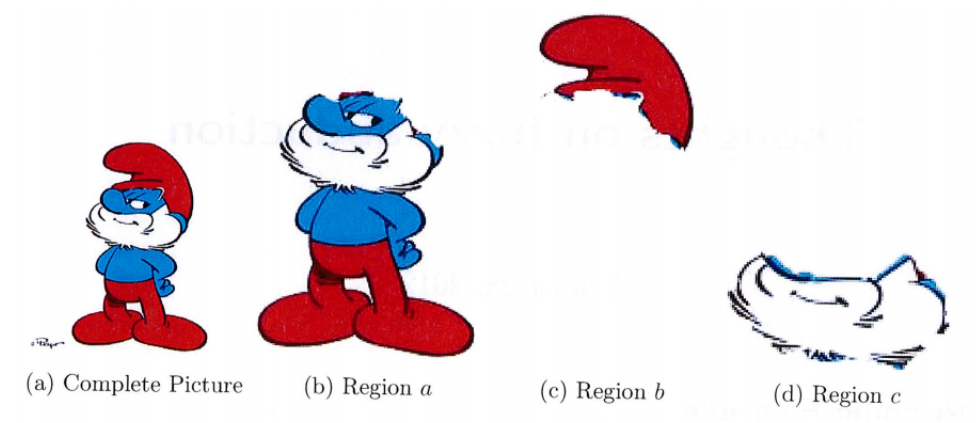
\includegraphics[scale=.3]{./figures/smurf.png}
   \caption{\label{fig:smurf}The smurf and its segmentation of different elements.}
 \end{figure} 
 
We illustrate this procedure with the image of the Smurf (Figure \ref{fig:smurf})\footnote{An example of abduction for interpretation of brain tumor is given in Appendix B}.
In the TBox, we describe the background knowledge that a leader smurf has a beard and wears a red hat as follows:
\begin{align*}
\mathcal{T}=\{SmurfLeader &\sqsubseteq \exists hasPart.Beard \sqcap \exists hasOnTop.RedHat, \\
RedHat &\equiv Hat \sqcap \exists hasColor.Red \} 
\end{align*}
Suppose that we can recognize three parts $a,b,c$ in an image and the observation is encoded by the following ABox:
\begin{align*}
\mathcal{A}_{obs} =\{(a,b)&: hasOnTop, \\
 (a,c)&: hasPart,\\
 b&:Hat,\\
 b&:\exists hasColor.Red,\\
 c&:Beard\}.
\end{align*}
Then, the most specific concept of $a$ is constructed as:
\begin{align*}
D=\exists hasPart.Beard \sqcap \exists hasOnTop.(Hat \sqcap  \exists hasColor.Red) 
\end{align*}

In our approach of the construction of the tableau, the initial node consists of two complex concepts.
One concept is satisfiable in $\mathbf{T}(1)$. Here, the concept is empty because we do not specify  a constraint.
The other is not satisfiable concept in $ \mathbf{F} (1) $. Here is the negation of the conjunction of $ C_\mathcal{T}$ and $ \neg O$. 

\begin{figure}
\centering
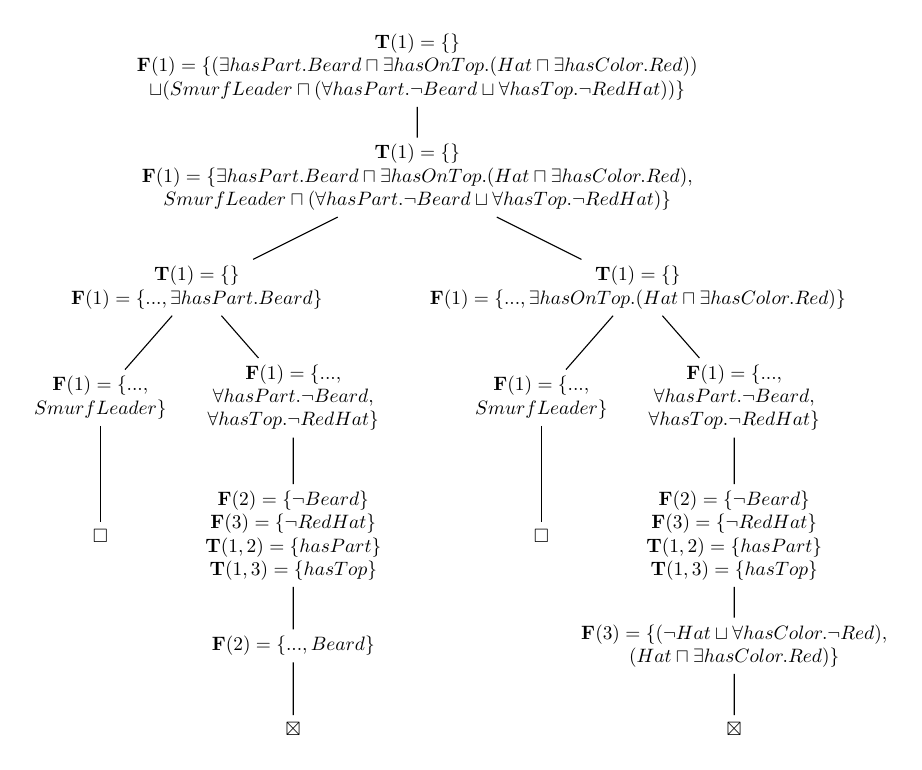
\begin{tikzpicture}[scale=0.7, transform shape,every text node part/.style={align=center},level 1/.style={level distance=2cm},level 2/.style={level distance=2cm, sibling distance=8cm},
level 3/.style={level distance=2cm,sibling distance=3.5cm},level 4/.style={level distance=2.5cm,sibling distance=2cm},level 5/.style={level distance=2cm},level 6/.style={level distance=1.5cm}]
\node [sibling distance=12cm] {$\mathbf{T}(1)=\{\}$ \\ $\mathbf{F}(1)=\{(\exists hasPart.Beard \sqcap \exists hasOnTop.(Hat \sqcap  \exists hasColor.Red))$ \\ $\sqcup (SmurfLeader \sqcap (\forall hasPart.\neg Beard \sqcup \forall hasTop. \neg RedHat)) \}$}
child { node []{$\mathbf{T}(1)=\{\}$ \\ $\mathbf{F}(1)=\{\exists hasPart.Beard \sqcap \exists hasOnTop.(Hat \sqcap  \exists hasColor.Red),$ \\ $SmurfLeader \sqcap (\forall hasPart.\neg Beard \sqcup \forall hasTop. \neg RedHat) \}$}
child { node []{$\mathbf{T}(1)=\{\}$ \\ $\mathbf{F}(1)=\{...,\exists hasPart.Beard  \}$}
	child { node []{$\mathbf{F}(1)=\{...,$\\$SmurfLeader \}$} 
			child{ node {$ \square $}}}
	child { node {$\mathbf{F}(1)=\{...,$\\$\forall hasPart.\neg Beard,$\\$\forall hasTop. \neg RedHat\}$} 
			child{ node[level distance=1cm] {$\mathbf{F}(2)=\{\neg Beard\}$\\$\mathbf{F}(3)=\{\neg RedHat\}$\\$\mathbf{T}(1,2)=\{hasPart\}$\\$\mathbf{T}(1,3)=\{hasTop\}$}
					child{ node[level distance=2cm] {$\mathbf{F}(2)=\{..., Beard\}$}
						   child{ node[level distance=1cm] {$ \boxtimes $}}}}}
}
child { node  []{$\mathbf{T}(1)=\{\}$ \\ $\mathbf{F}(1)=\{..., \exists hasOnTop.(Hat \sqcap  \exists hasColor.Red)\}$}
	child { node {$\mathbf{F}(1)=\{...,$\\$SmurfLeader \}$} 
			child{ node {$ \square $}}}
	child { node {$\mathbf{F}(1)=\{...,$\\$\forall hasPart.\neg Beard,$\\$\forall hasTop. \neg RedHat\}$}
			child{ node[level distance=1cm] {$\mathbf{F}(2)=\{\neg Beard\}$\\$\mathbf{F}(3)=\{\neg RedHat\}$\\$\mathbf{T}(1,2)=\{hasPart\}$\\$\mathbf{T}(1,3)=\{hasTop\}$}
					child{ node[level distance=2cm] {$\mathbf{F}(3)=\{(\neg Hat \sqcup  \forall hasColor.\neg Red),$\\$ (Hat \sqcap  \exists hasColor.Red)\}$}
						   child{ node[level distance=1cm] {$ \boxtimes $}}}} }
}
};

\end{tikzpicture}
\caption{The process of constructing the tableau by applying expansion rules.}\label{fig:grandst}
\end{figure}

By applying expansion rules, the construction process of the tableau is shown in Figure \ref{fig:grandst}. The hypotheses are generated from open branches.
In this example, we have two sets of concepts:
% Puis, nous pouvons générer un ensemble de concepts non décomposables pour chaque branche ouverte. Un concept qui ne peut subir aucune règle d'expansion est appelé non décomposable.
% Dans cet exemple, nous avons deux ensembles:
\begin{align*}
H_1&=\{SmurfLeader,~\exists hasPart.Beard\}\\
H_2&=\{SmurfLeader,~\exists hasOnTop.(Hat \sqcap  \exists hasColor.Red)\}
\end{align*}
The concepts in these two sets are basic elements to build a hypothesis $H$. The hypothesis $H$ is considered as a concept in $\mathbf{T}(1)$.
To close the tableau, we can take these concepts in $\mathbf{F}(1)$ to generate a heterogeneous clash.
The first branch is closed if one takes the concept $SmurfLeader$, $\exists hasPart.Beard$ or the combination of these two concepts
$SmurfLeader \sqcap \exists hasPart.Beard$. The concept $SmurfLeader$ is also a concept for closing the second branch. We can then consider that $H\equiv SmurfLeader$
is a potential hypothesis. Apart from this case, $\exists hasPart. Beard \sqcap \exists hasOnTop.(Hat \sqcap \exists hasColor.Red)$,
$SmurfLeader \sqcap \exists hasOnTop.(Hat \sqcap \exists hasColor.Red)$, $SmurfLeader \sqcap \exists hasPart.Beard$ are also potential hypotheses.

% \subsubsection{Tableau closure (minimal hitting set)}
At this stage, we conducted a construction procedure of the tree model using  the tableau method. Then we have a set of concepts for each open branch in the tableau.
One potential hypothesis is the combination of these concepts. The considered concepts can close the table if at least one concept is selected in each branch.
To avoid redundancy, we want to take the minimum hitting set. 
\begin{mydef}{(Hitting set)}
 Let $\{ S_1,\dots,S_n\}$ be a collection of sets. A hitting set  $T$ is a subset $T\subseteq \cup_{i=1}^{n} S_i$ such that $T$ contains at least one element
 of each set in the collection $T \cap S_i \neq \emptyset~(1\leq i\leq n)$.
 The minimal hitting set is a hitting set $T_m$ if  $\nexists$ hitting set $T'$ such that $T'\subset T_m$.
\end{mydef}

Such a minimal hitting set of concepts guarantees a syntactical hypothesis in the given DL. 
To ensure the consistency and relevance of an explanation, the following properties are required to be satisfied for each potential hypothesis:
\begin{description}
 \item[\textbf{Relevant}] $\mathcal{K}\vDash \mathcal{H} \sqsubseteq \mathcal{O}$
 \item[\textbf{Consistent}] $\mathcal{K},\mathcal{H} $ are consistent.
 \item[\textbf{Explainable}] $\mathcal{K},\nvDash \mathcal{O}, \mathcal{H}   \nvDash \mathcal{O}$
\end{description}
\medskip

% Une approche exhaustive est proposée dans l'algorithme~\ref{exhaustive}:
An exhaustive algorithm is proposed for selecting the minimal hitting set:

\begin{algorithm}[H]
\textbf{Input:} A collection of sets $\{S_1,\dots,S_n\}$\;
\textbf{Output:} A collection of hitting sets $\mathcal{H}$\;
Initialization\:
$\mathcal{H}=\{\}$\;
Root initialization.\;
\textbf{For~}( $i$ From 1 to $n$ )\textbf{~do:}\\
~~~~~~Create a new leaf for every  $S_i$  in each branch\;
~~~~~~An intermediate hypothesis $H_{j}$ is the conjunction of all the concepts in the same branch\;
~~~~~~Delete the branch $j$ if $H_{j}$ is inconsistent w.r.t. the TBox\;
\textbf{End}\\
The conjunction of all concepts in each branch $j$ represents a potential hypothesis $H_j$\;
\textbf{return:} $\mathcal{H}$\;
\caption{Exhaustive search algorithm of selecting hitting sets.}\label{algo:exhaustive}
\end{algorithm}


\begin{figure}
\centering
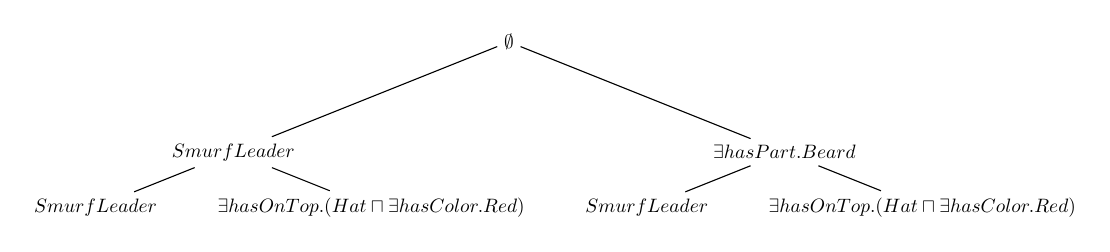
\begin{tikzpicture}[scale=0.7, transform shape, every text node part/.style={align=center},level 1/.style={level distance=2cm,sibling distance=10cm},level 2/.style={level distance=1cm, sibling distance=5cm}]
\node [sibling distance=12cm] {$\emptyset$}
child { node []{$SmurfLeader$}
     child{ node []{$SmurfLeader$}}
     child{ node []{$\exists hasOnTop.(Hat \sqcap  \exists hasColor.Red)$}}
}
child { node  []{$\exists hasPart.Beard$}
     child{ node []{$SmurfLeader$}}
     child{ node []{$\exists hasOnTop.(Hat \sqcap  \exists hasColor.Red)$}}
};

\end{tikzpicture}
\caption{Hitting set construction tree.\label{fig:hittingtree}}
\end{figure}
We illustrate the algorithm by the example of Smurf. Note that we got two sets of concepts in the previous step.
Applying this algorithm, a tree is initialized with an empty root. Then we construct recursively the tree by adding all concepts
in the set $h_i$ as new leaves (Figure \ref{fig:hittingtree}). In this case, all
assumptions are consistent with the TBox:
$H_1=SmurfLeader$, $H_2=\exists hasPart.Beard \sqcap \exists hasOnTop.(Hat\sqcap\exists hasColor.Red)$, 
$H_3=SmurfLeader\sqcap\exists hasOnTop.(Hat\sqcap \exists hasColor.Red)$, $H_4=SmurfLeader \sqcap \exists hasPart.Beard$. 
The second hypothesis is removed because $H=\exists hasPart.Beard \sqcap \exists hasOnTop.(Hat\sqcap\exists hasColor.Red)$ 
is not an independent explainable hypothesis ($H\vDash \mathcal{O}$). 

Assumptions made in this algorithm are consistency and syntactical minimality. 
A preference explanation depends on a minimality criterion that will be presented in the next subsection.

\subsection{Minimality criteria}
Abduction can be also defined as inference to the best explanation.
A set of potential hypotheses is generated based on the tableau method. However, only a part of them can be selected according to the defined preference by filtering inconsistent and redundant ones. 
One potential hypothesis is an explanation if and only if the requirements in the previous section are fulfilled to avoid irrelevant results and observations themselves.
The preference relies on different kinds of minimality criteria. 
In~\cite{bienvenu08complexity}, Bienvenu provided five basic criteria for abduction problems.
An abduction problem is defined as: $ \langle \mathcal{T}, \mathcal{H}, \mathcal{O}\rangle$, where $\mathcal{T}$ is a TBox, $\mathcal{H}$ is a set of atomic concepts and $\mathcal{O}$ is the observed concept.

\begin{mydef}{(Explanation~\cite{bienvenu08complexity})}
$\{ A_1,\dots,A_n \} \subseteq \mathcal{H}$ is a subset of $\mathcal{H}$. An explanation of abduction problem $ \langle \mathcal{T}, \mathcal{H}, \mathcal{O}\rangle$ can be formulated from the set if:
\begin{itemize}
\item  $A_1 \sqcap \dots \sqcap A_n$ is satisfiable w.r.t. $\mathcal{T}$.
\item $\mathcal{T}  \vDash  A_1 \sqcap \dots \sqcap A_n \sqsubseteq \mathcal{O}$
\end{itemize}

\end{mydef}

In this problem, an hypothesis is formulated with the conjunction of atomic concepts.
Five minimality criteria are then defined as follows.
\begin{mydef}{(Minimality criteria~\cite{bienvenu08complexity})}
For an abduction problem $\mathcal{P}=\langle \mathcal{T},\mathcal{H}, \mathcal{O}\rangle$, $\mathcal{A}=\{H_1,\dots,$ $H_n \} \subseteq \mathcal{H}$ is an explanation of the problem $\mathcal{P}$,
$\langle H_{(1)},\dots,H_{(n)}\rangle$ is a priority order of  $\mathcal{H}$,
and $w:\mathcal{H}\rightarrow \mathbb{N}$ is a weighting function to defining the importance of the hypotheses. The criteria can be defined as follows:
\begin{itemize}
\item  $\mathcal{A}~$ is  $~\subseteq -minimal$ if there does not exist an explanation $\mathcal{B}$ for $\mathcal{P}$ such that $\mathcal{B} \subsetneq \mathcal{A}$,
\item  $\mathcal{A}~$ is  $~\leq -minimal$ if there does not exist an explanation $\mathcal{B}$ for $\mathcal{P}$ such that $\abs{\mathcal{B}} < \abs{\mathcal{A}}$,
\item  $\mathcal{A}~$ is  $~\subseteq_P -minimal$ if there does not exist an explanation $\mathcal{B}$ for $\mathcal{P}$ such that $\mathcal{B} \cap H_i \subsetneq \mathcal{A}\cap H_i$ and
$\mathcal{B} \cap H_j = \mathcal{A}\cap H_j$ where $1\leq j< i$,
\item  $\mathcal{A}~$ is  $~\leq_P -minimal$ if there does not exist an explanation $\mathcal{B}$ for $\mathcal{P}$ such that $\abs{\mathcal{B} \cap H_i} < \abs{\mathcal{A}\cap H_i}$ and
$\abs{\mathcal{B} \cap H_j} = \abs{\mathcal{A}\cap H_j}$ where $1\leq j< i$,
\item  $\mathcal{A}~$ is  $~\sqsubseteq_w -minimal$ if there does not exist an explanation $\mathcal{B}$ for $\mathcal{P}$ such that $\sum_{B \in \mathcal{B}}w(B) < \sum_{A \in \mathcal{A}}w(A)$.
\end{itemize}
 \end{mydef}

 \begin{mydef}{(Subsumption criterion)}
For an abduction problem $\mathcal{P}=\langle \mathcal{T},\mathcal{H}, \mathcal{O}\rangle$, and $\{\langle P_{1},\dots,P_{n}\rangle\}$ potential hypotheses,
\begin{itemize}
\item  $P_{i}$ is a $\bm{\sqsubseteq -minimal}$ explanation if there does not exist an explanation $P_{j}$ for $\mathcal{P}$ such that $P_{i}\sqsubseteq P_{j}$.
\end{itemize}
\end{mydef}
For example, let us consider $Father \sqcap \exists hasChild.Person \sqsubseteq Man$. The concept $\exists hasChild.Person$ can be inferred from $Father$.
Therefore, $\exists hasChild.Person$ is the redundant part which can be eliminated. 

Another specific criterion mentioned in \cite{di2007semantic} is dedicated to the matchmaking application,
The authors proposed an irreducible-minimum criterion in their formalism.
An irreducible solution is represented in conjunctive normal form where complex concepts are replaced by the conjunction of super concept
considering GCI axioms in the TBox.
This model of the explanation is suitable for matchmaking applications, however, it is an explanation with little information in our traditional cases.

However, we can adapt this test to our problem. We can then calculate the cardinality of the irreducible results for comparison.
We can represent concepts in conjunctive normal form (CNF) to the assumptions and observation. As the assumption is subsumed by the observation, connective concepts of hypothesis are a subset
those of observation. We present a metric function $ f_{ranking}$  to assess the quality that assumption. Here, one can calculate the cardinality of the different part
between the hypothesis and observation. The concept with the least difference to other assumptions is preferred as an irreducible minimum explanation. Can also
assign a value to each concept and calculate the weighting for the different part.

\begin{mydef}{(Irreducible criterion)}
For an abduction problem $\mathcal{P}=\langle \mathcal{T},\mathcal{H}, \mathcal{O}\rangle$, and $\{\langle P_{1},\dots,P_{n}\rangle\}$ are potential hypotheses,
\begin{itemize}
\item  $P_{i}$ is an $\bm{irreductible-minimal}$ explanation if there does not exist an explanation $P_{j}$ for $\mathcal{P}$ such that $f_{ranking}(\mathcal{T},FNC(P_{j}),FNC(\mathcal{O})) 
< f_{ranking}(\mathcal{T},FNC(P_{i}),FNC(\mathcal{O}))$.
\end{itemize}
\end{mydef}
In the example of interpretation of the Smurf, the explanation $H_1=SmurfLeader$ is the ``best'' explanation according to all the criteria presented
in this section.

The criteria introduced by Bienvenu are useful when an assumption contains only atomic concepts. It considers that a hypothesis is constructed by the conjunction of atomic concepts.
The criterion concerns inclusion relations of set theory, possibly with the priority and the weight function.
In our problem, a hypothesis can be made by non-atomic concepts. The subsumption test is a good choice in many works,
for example those of Colucci \textit{et al.} \cite{colucci2004uniform} and those of Atif \textit{et al.}  \cite{atif2014explanatory}. 
The hierarchical relationship is considered to seek a more general hypothesis.
The irreducibility criterion is a criterion combining a criterion of subsumption and a criterion of cardinality. This criterion has the advantage that the measure $f_{ranking}$  can be adapted to different measures.
For example, if we apply the abduction in fuzzy logic, a degree of possibility can be considered as a practical measure.

\section{Perspectives}\label{sec:persp}
During the first part of the thesis, we have exploited Description Logics and associated tableau method for knowledge representation and reasoning in image interpretation.
A first model of background knowledge of brain anatomy  including spatial information is proposed.  
At this stage, we have adapted the tableau method for generating preferred hypotheses w.r.t. the TBox.

Several directions will be considered in the next step.
A work in the first place is to generate adaptive hypotheses iteratively.
We have demonstrated that the tableau method produces a large amount of hypotheses, however, most of them are irrelevant or unsatisfiable.
In order to avoid getting these hypotheses, an iterative method is considered.
Instead of adding all internalized concepts into the tableau, we add only the ones corresponding to relative axioms in which observed concepts occurring.
This part will be explored in detail and be prepared for a submission to an international conference.


Concrete domains are necessary in image interpretation by providing an interface between abstract logical level and concrete image space,
because semantic truth models may not have corresponding regions in concrete domains.
For example, a concept $CNl\sqcap \exists rightOf CNr$ could be verified to be satisfiable w.r.t. to a defined TBox.
However, this concept may not have a model in the image space.

Fuzzy logic is also a useful ingredient in knowledge representation dealing with imprecision and vague information.
This aspect has been proved to be expressive for spatial reasoning by combining fuzzy relations in the concrete domains to Description Logics for image interpretation~\cite{hudelot2008spatial}.
Another strategy to integrate fuzzy set theory into knowledge representation is to add fuzzy value to terminological and assertional knowledge in abstract logical level.
This part of the work will allow dealing directly with satisfaction degrees of spatial relations (without thresholding them).


As we have discussed in Section \ref{sec:qsr}, we have considered spatial relations in a more complex way without approximating an object to a single point,
Therefore, qualitative spatial reasoning remains an open problem, especially including topological relations and their compositions in abductive reasoning services for the aim of image interpretation.
This will be an important part of the thesis.

\section{Other Activities}
During the first half of my thesis, I also participated in different activities in the TII group and TAO group 
in LRI\footnote{Laboratoire de Recherche en Informatique, Universit\'{e} ParisSud}.
\begin{itemize}
 \item I presented my work in the meetings of the ANR project LOGIMA\footnote{\url{http://logima.gforge.inria.fr/doku.php}}.
 \item I presented my work in the seminars of the group.
 \item I have taken doctoral courses in EDITE\footnote{\url{http://edite-de-paris.fr/spip/}}
 (Formations in French: Rendre des articles attractifs, Intelligence Economique, Brevets, Pratique de la négociation de projet à l'international).
\end{itemize}

\appendix
\section{An illustrative example using $\mathcal{ALCHI_{R_+}}$ tableau method}
\label{Appendix A}

This example can be treated as an abductive reasoning involving qualitative spatial relations.
The example is illustrated according to the knowledge base in Section \ref{sec:qsr}.
The reasoning concerned about testing the subsumption between a potential hypothesis $H\equiv LVl\sqcap \exists isPartOf.Hemisphere$ and an observed concept.
The observed concept is represented by the most specific concept (see Definition \ref{def:msc}) of  $b^\mathcal{I}$
($O\equiv \exists (leftOf^-\sqcap closeTo^-). CNl\sqcap \exists isPartOf.Brain$ and $H\equiv LVl\sqcap \exists isPartOf.Hemisphere$).
To check subsumption of the two concepts $H$ and $O$, $\mathcal{K} \vDash H\sqcap \neg O \sqsubseteq \bot$ is required to prove that $H\sqcap \neg O$ is unsatisfiable.
Let $x$ be the interpretation element of the concept $H\sqcap \neg O$.


The tableau is initialized with $\mathcal{L}(x)=\{ LVl\sqcap \exists isPartOf.Hemisphere\sqcap \forall (leftOf^-\sqcap closeTo^-).\neg CNl\sqcup \forall isPartOf.\neg Brain\}$.
In the first step, $\sqcap$ and $\sqcup$ rule (Rule 2 and Rule 3) are applied and we obtain:
\begin{center}
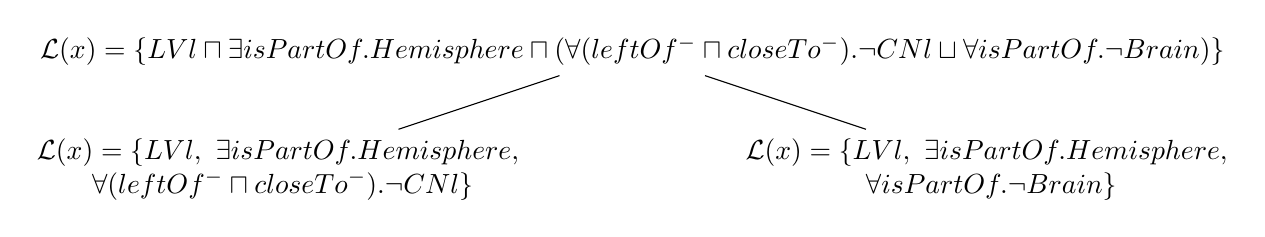
\begin{tikzpicture}[every text node part/.style={align=center},level 1/.style={level distance=1.5cm, sibling distance=9cm}]
\node [sibling distance=18cm] {$\mathcal{L}(x)=\{ LVl\sqcap \exists isPartOf.Hemisphere\sqcap (\forall (leftOf^-\sqcap closeTo^-).\neg CNl\sqcup \forall isPartOf.\neg Brain)\}$}
	      child{ node {$\mathcal{L}(x)=\{ LVl,~\exists isPartOf.Hemisphere,$\\$~\forall (leftOf^-\sqcap closeTo^-).\neg CNl\}$}}
	      child{ node {$\mathcal{L}(x)=\{ LVl,~\exists isPartOf.Hemisphere,$\\$~\forall isPartOf.\neg Brain\}$}};
\end{tikzpicture} 
\end{center}

To include the terminological knowledge, axioms like $C\sqsubseteq D$ in the TBox can be internalized into single concepts ($\neg C\sqcup D$) and added to $\mathcal{L}(x)$. Here, for the sake of simplicity 
of demonstration, we only add the internalization of the axiom $LVl \sqsubseteq BrainStructure \sqcap  \exists (rightOf \sqcap closeTo). CNl$ for the first branch.
\begin{center}
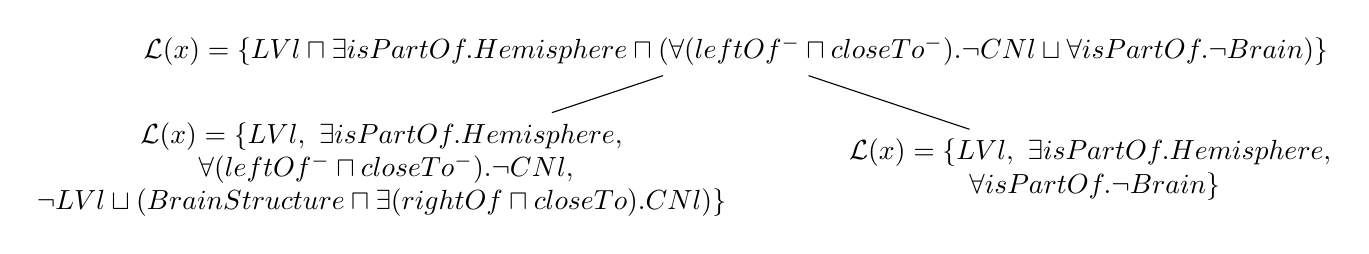
\begin{tikzpicture}[every text node part/.style={align=center},level 1/.style={level distance=1.5cm, sibling distance=9cm}]
\node [sibling distance=18cm] {$\mathcal{L}(x)=\{ LVl\sqcap \exists isPartOf.Hemisphere\sqcap (\forall (leftOf^-\sqcap closeTo^-).\neg CNl\sqcup \forall isPartOf.\neg Brain)\}$}
	      child{ node {$\mathcal{L}(x)=\{ LVl,~\exists isPartOf.Hemisphere,$\\$~\forall (leftOf^-\sqcap closeTo^-).\neg CNl,$\\$\neg LVl \sqcup (BrainStructure \sqcap \exists (rightOf \sqcap closeTo).CNl)\}$}}
	      child{ node {$\mathcal{L}(x)=\{ LVl,~\exists isPartOf.Hemisphere,$\\$~\forall isPartOf.\neg Brain\}$}};
\end{tikzpicture}  
\end{center}

We then apply $\sqcap$ and $\sqcup$ rule (Rule 2 and Rule 3) again on the first branch:
\begin{center}
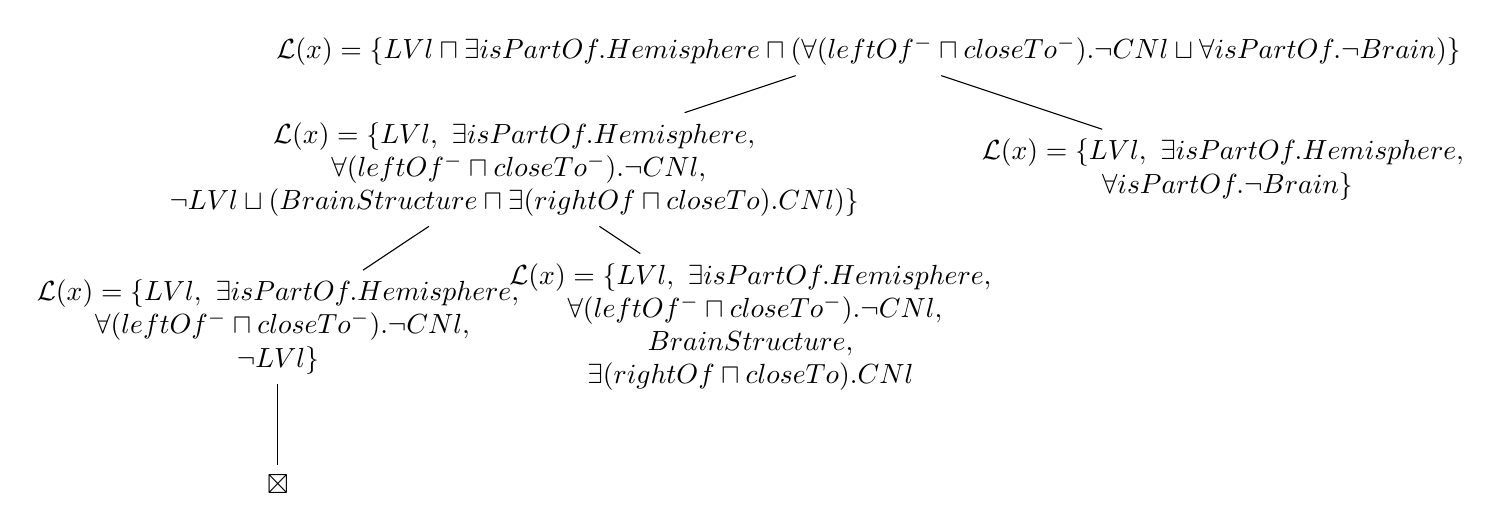
\begin{tikzpicture}[every text node part/.style={align=center},level 1/.style={level distance=1.5cm, sibling distance=9cm}, level 2/.style={level distance=2cm, sibling distance=6cm}]
\node [sibling distance=18cm] {$\mathcal{L}(x)=\{ LVl\sqcap \exists isPartOf.Hemisphere\sqcap (\forall (leftOf^-\sqcap closeTo^-).\neg CNl\sqcup \forall isPartOf.\neg Brain)\}$}
	      child{ node {$\mathcal{L}(x)=\{ LVl,~\exists isPartOf.Hemisphere,$\\$~\forall (leftOf^-\sqcap closeTo^-).\neg CNl,$\\$\neg LVl \sqcup (BrainStructure \sqcap \exists (rightOf \sqcap closeTo).CNl)\}$}
	      		    child{ node {$\mathcal{L}(x)=\{ LVl,~\exists isPartOf.Hemisphere,$\\$~\forall (leftOf^-\sqcap closeTo^-).\neg CNl,$\\$\neg LVl\}$}
				  child{ node{$\boxtimes$}}}
		            child{ node {$\mathcal{L}(x)=\{ LVl,~\exists isPartOf.Hemisphere,$\\$~\forall (leftOf^-\sqcap closeTo^-). \neg CNl,$\\$BrainStructure,$\\$\exists (rightOf \sqcap closeTo).CNl$}}}
	      child{ node {$\mathcal{L}(x)=\{ LVl,~\exists isPartOf.Hemisphere,$\\$~\forall isPartOf.\neg Brain\}$}};
\end{tikzpicture}  
\end{center}

A clash ($LVl,~\neg LVl$) is detected in the first part of the first branch (closed). We then apply $\exists$ rule (Rule 4) on the second part:
\begin{center}
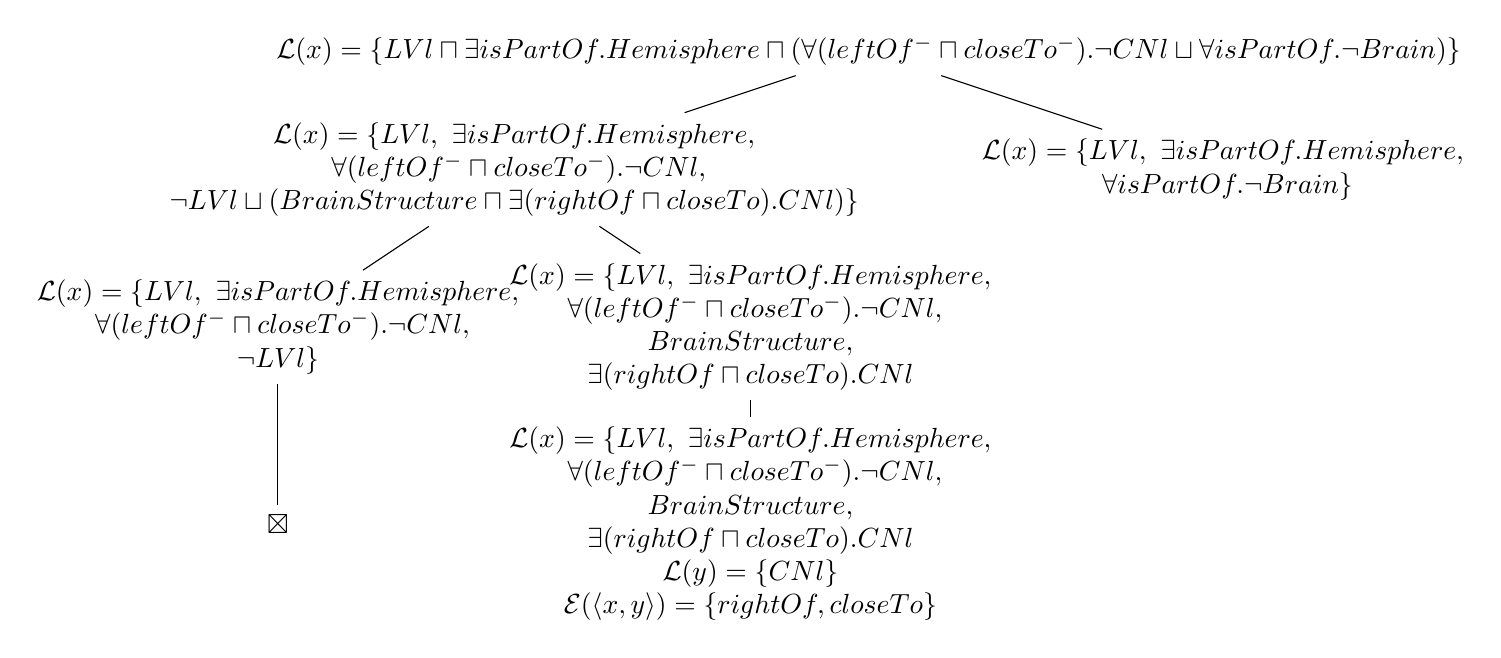
\begin{tikzpicture}[every text node part/.style={align=center},level 1/.style={level distance=1.5cm, sibling distance=9cm}, level 2/.style={level distance=2cm, sibling distance=6cm},
level 3/.style={level distance=2.5cm, sibling distance=6cm}]
\node [sibling distance=18cm] {$\mathcal{L}(x)=\{ LVl\sqcap \exists isPartOf.Hemisphere\sqcap (\forall (leftOf^-\sqcap closeTo^-).\neg CNl\sqcup \forall isPartOf.\neg Brain)\}$}
	      child{ node {$\mathcal{L}(x)=\{ LVl,~\exists isPartOf.Hemisphere,$\\$~\forall (leftOf^-\sqcap closeTo^-).\neg CNl,$\\$\neg LVl \sqcup (BrainStructure \sqcap \exists (rightOf \sqcap closeTo).CNl)\}$}
	      		    child{ node {$\mathcal{L}(x)=\{ LVl,~\exists isPartOf.Hemisphere,$\\$~\forall (leftOf^-\sqcap closeTo^-).\neg CNl,$\\$\neg LVl\}$}
				  child{ node{$\boxtimes$}}}
		            child{ node {$\mathcal{L}(x)=\{ LVl,~\exists isPartOf.Hemisphere,$\\$~\forall (leftOf^-\sqcap closeTo^-).\neg CNl,$\\$BrainStructure,$\\$\exists (rightOf \sqcap closeTo).CNl$}
				  child{ node {$\mathcal{L}(x)=\{ LVl,~\exists isPartOf.Hemisphere,$\\
				  $~\forall (leftOf^-\sqcap closeTo^-).\neg CNl,$\\$BrainStructure,$\\$\exists (rightOf \sqcap closeTo).CNl$\\
				  $\mathcal{L}(y)=\{CNl\}$\\
				  $\mathcal{E}(\langle x,y \rangle)=\{rightOf,closeTo\}$}}}}
	      child{ node {$\mathcal{L}(x)=\{ LVl,~\exists isPartOf.Hemisphere,$\\$~\forall isPartOf.\neg Brain\}$}};
\end{tikzpicture}  
\end{center}

Because of inverse role axiom in the RBox, we can add inverse roles in $\mathcal{E}(\langle x,y \rangle)$ (Rule 7) and apply  $\forall$ rule (Rule 5) on the second part:
\begin{center}
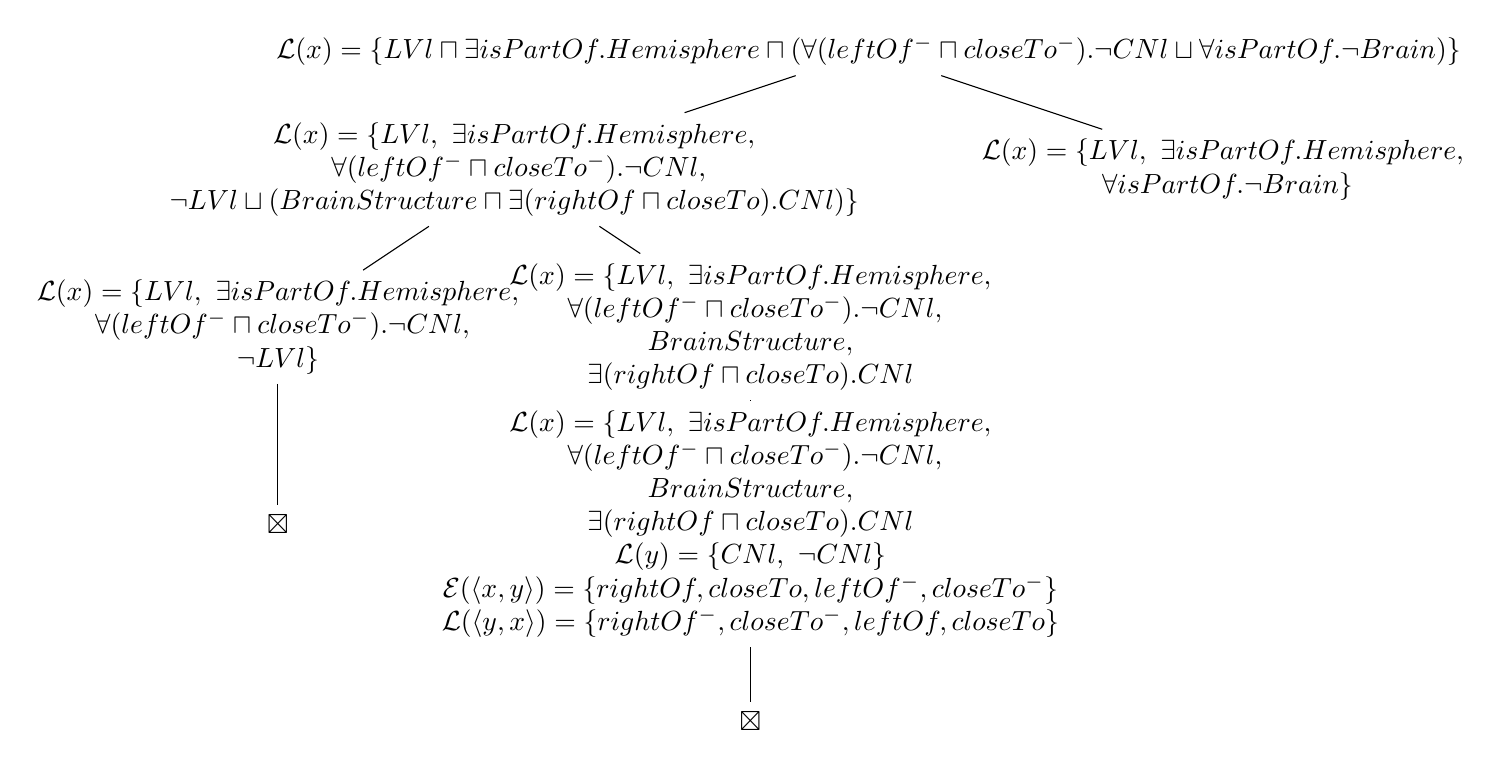
\begin{tikzpicture}[every text node part/.style={align=center},level 1/.style={level distance=1.5cm, sibling distance=9cm}, level 2/.style={level distance=2cm, sibling distance=6cm},
level 3/.style={level distance=2.5cm, sibling distance=6cm}]
\node [sibling distance=18cm] {$\mathcal{L}(x)=\{ LVl\sqcap \exists isPartOf.Hemisphere\sqcap (\forall (leftOf^-\sqcap closeTo^-).\neg CNl\sqcup \forall isPartOf.\neg Brain)\}$}
	      child{ node {$\mathcal{L}(x)=\{ LVl,~\exists isPartOf.Hemisphere,$\\$~\forall (leftOf^-\sqcap closeTo^-).\neg CNl,$\\$\neg LVl \sqcup (BrainStructure \sqcap \exists (rightOf \sqcap closeTo).CNl)\}$}
	      		    child{ node {$\mathcal{L}(x)=\{ LVl,~\exists isPartOf.Hemisphere,$\\$~\forall (leftOf^-\sqcap closeTo^-).\neg CNl,$\\$\neg LVl\}$}
				  child{ node{$\boxtimes$}}}
		            child{ node {$\mathcal{L}(x)=\{ LVl,~\exists isPartOf.Hemisphere,$\\$~\forall (leftOf^-\sqcap closeTo^-).\neg CNl,$\\$BrainStructure,$\\$\exists (rightOf \sqcap closeTo).CNl$}
				  child{ node {$\mathcal{L}(x)=\{ LVl,~\exists isPartOf.Hemisphere,$\\
				  $~\forall (leftOf^-\sqcap closeTo^-).\neg CNl,$\\$BrainStructure,$\\$\exists (rightOf \sqcap closeTo).CNl$\\
				  $\mathcal{L}(y)=\{CNl,~\neg CNl\}$\\
				  $\mathcal{E}(\langle x,y \rangle)=\{rightOf,closeTo,leftOf^-,closeTo^-\}$\\
				  $\mathcal{L}(\langle y,x\rangle)=\{rightOf^-,closeTo^-,leftOf,closeTo\}$}
				  child{ node{$\boxtimes$}}}}}
	      child{ node {$\mathcal{L}(x)=\{ LVl,~\exists isPartOf.Hemisphere,$\\$~\forall isPartOf.\neg Brain\}$}};
\end{tikzpicture}  
\end{center}

The first branch of the tableau is closed because of the clash of $CNl$ and $\neg CNl$ in the second part.
We then explore the second branch. At first we apply the $\exists$ rule (Rule 4) and then $\forall$ rule (Rule 5):
\begin{center}
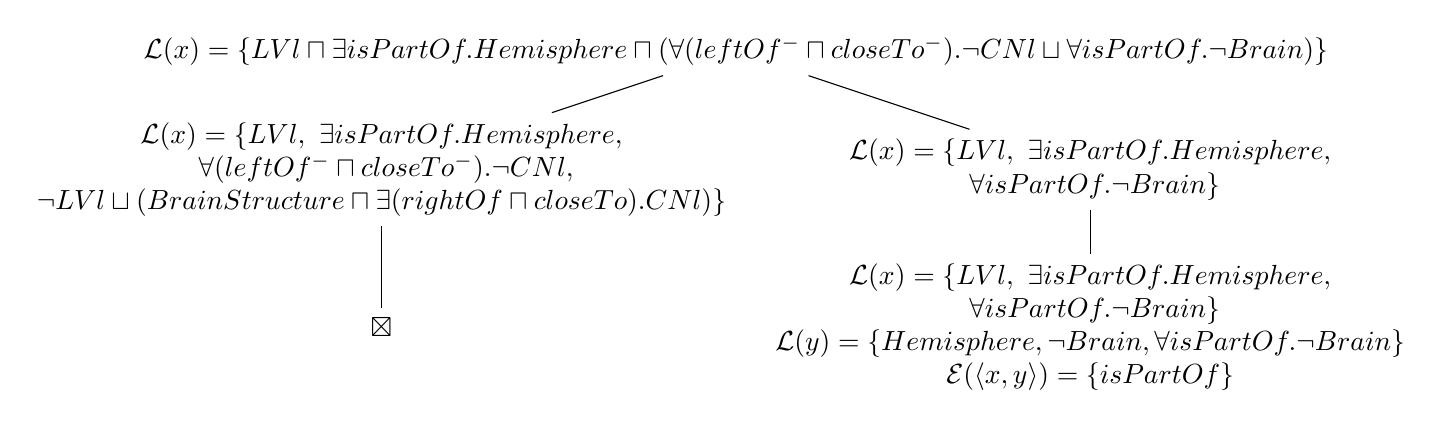
\begin{tikzpicture}[every text node part/.style={align=center},level 1/.style={level distance=1.5cm, sibling distance=9cm}, level 2/.style={level distance=2cm, sibling distance=6cm},
level 3/.style={level distance=2.5cm, sibling distance=6cm}]
\node [sibling distance=18cm] {$\mathcal{L}(x)=\{ LVl\sqcap \exists isPartOf.Hemisphere\sqcap (\forall (leftOf^-\sqcap closeTo^-).\neg CNl\sqcup \forall isPartOf.\neg Brain)\}$}
	      child{ node {$\mathcal{L}(x)=\{ LVl,~\exists isPartOf.Hemisphere,$\\$~\forall (leftOf^-\sqcap closeTo^-).\neg CNl,$\\$\neg LVl \sqcup ( BrainStructure \sqcap \exists (rightOf \sqcap closeTo).CNl)\}$}
				  child{ node{$\boxtimes$}}}
	      child{ node {$\mathcal{L}(x)=\{ LVl,~\exists isPartOf.Hemisphere,$\\$~\forall isPartOf.\neg Brain\}$}
		     child{ node{$\mathcal{L}(x)=\{ LVl,~\exists isPartOf.Hemisphere,$\\$~\forall isPartOf.\neg Brain\}$\\
				  $\mathcal{L}(y)=\{ Hemisphere, \neg Brain, \forall isPartOf. \neg Brain\}$\\
				  $\mathcal{E}(\langle x,y \rangle)=\{isPartOf\}$}}};
\end{tikzpicture}  
\end{center}

The axiom $Hemisphere \sqsubseteq \exists isPartOf.Brain$ is internalized and added into $\mathcal{L}(y)$. Then we continue to extend the second branch with expansion rules (Rules 2,3,4,6,7):
\begin{center}
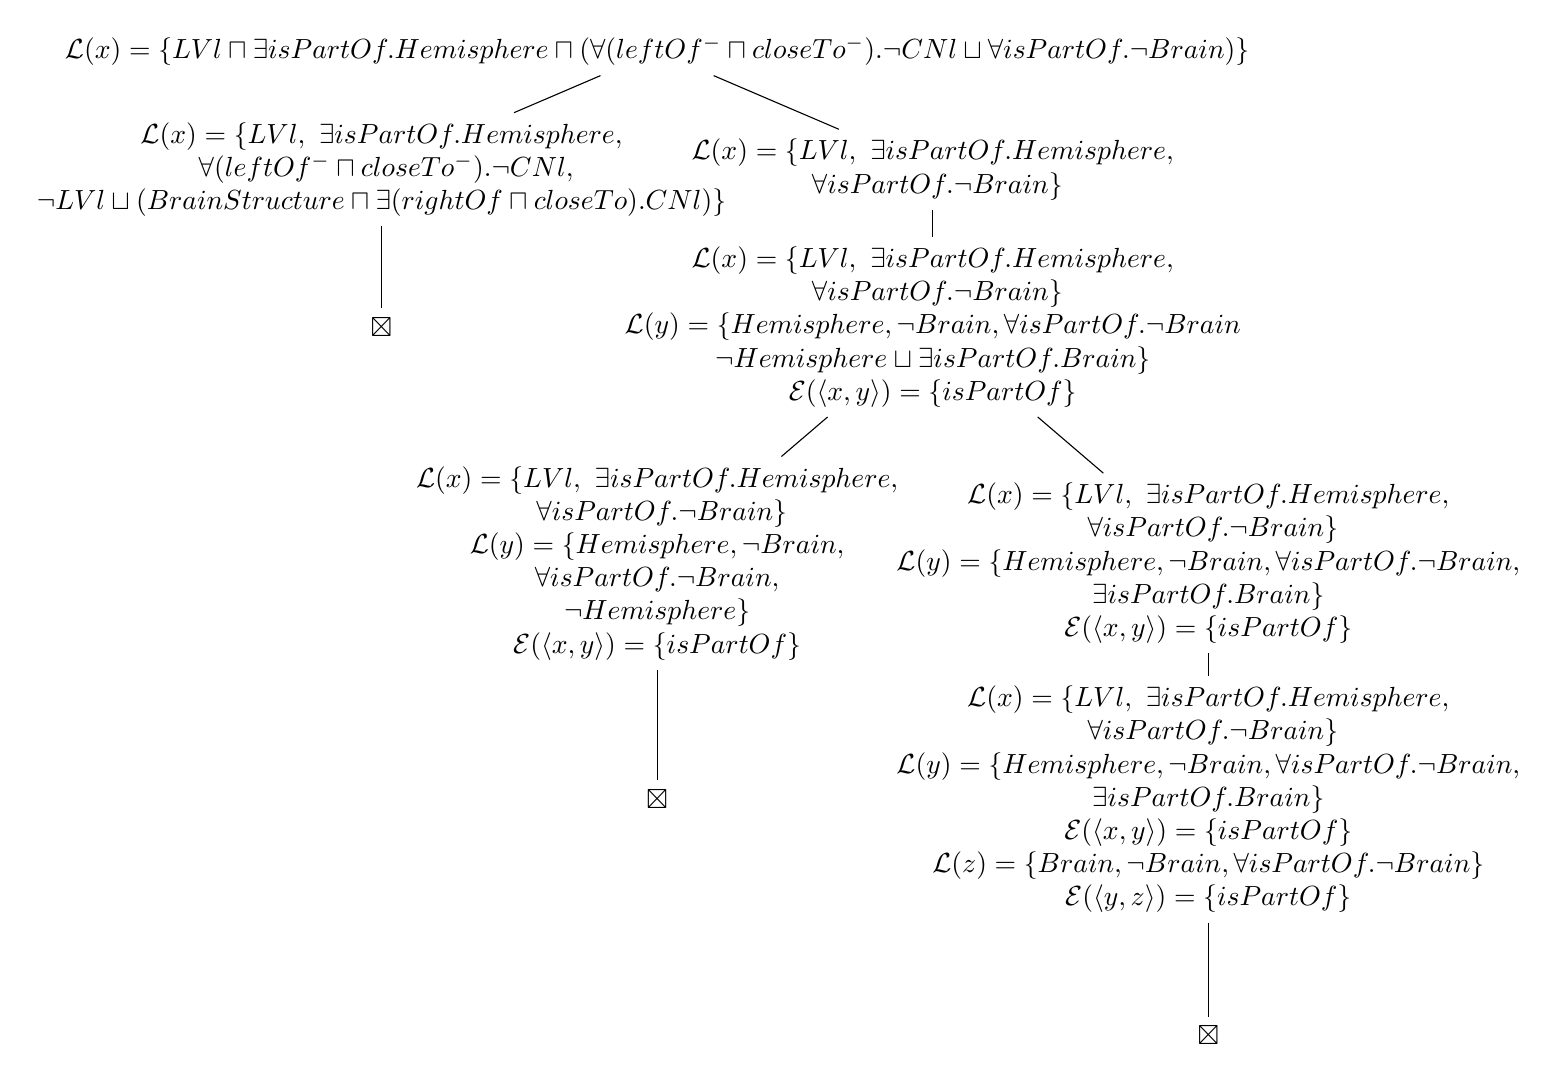
\begin{tikzpicture}[every text node part/.style={align=center},level 1/.style={level distance=1.5cm, sibling distance=7cm}, level 2/.style={level distance=2cm, sibling distance=6cm},
level 3/.style={level distance=3cm, sibling distance=7cm}]
\node [sibling distance=18cm] {$\mathcal{L}(x)=\{ LVl\sqcap \exists isPartOf.Hemisphere\sqcap ( \forall (leftOf^-\sqcap closeTo^-).\neg CNl\sqcup \forall isPartOf.\neg Brain)\}$}
	      child{ node {$\mathcal{L}(x)=\{ LVl,~\exists isPartOf.Hemisphere,$\\$~\forall (leftOf^-\sqcap closeTo^-).\neg CNl,$\\$\neg LVl \sqcup( BrainStructure \sqcap \exists (rightOf \sqcap closeTo).CNl)\}$}
				  child{ node{$\boxtimes$}}}
	      child{ node {$\mathcal{L}(x)=\{ LVl,~\exists isPartOf.Hemisphere,$\\$~\forall isPartOf.\neg Brain\}$}
		     child{ node{$\mathcal{L}(x)=\{ LVl,~\exists isPartOf.Hemisphere,$\\$~\forall isPartOf.\neg Brain\}$\\
				  $\mathcal{L}(y)=\{ Hemisphere, \neg Brain, \forall isPartOf. \neg Brain$\\
				  $\neg Hemisphere \sqcup \exists isPartOf.Brain\}$\\
				  $\mathcal{E}(\langle x,y \rangle)=\{isPartOf\}$}
				  child{ node{$\mathcal{L}(x)=\{ LVl,~\exists isPartOf.Hemisphere,$\\$~\forall isPartOf.\neg Brain\}$\\
					      $\mathcal{L}(y)=\{ Hemisphere, \neg Brain,$\\$ \forall isPartOf. \neg Brain,$\\
					      $\neg Hemisphere\}$\\
					      $\mathcal{E}(\langle x,y \rangle)=\{isPartOf\}$ }
					      child{ node{$\boxtimes$}}}
				  child{ node{$\mathcal{L}(x)=\{ LVl,~\exists isPartOf.Hemisphere,$\\$~\forall isPartOf.\neg Brain\}$\\
					      $\mathcal{L}(y)=\{ Hemisphere, \neg Brain, \forall isPartOf. \neg Brain$,\\
					      $ \exists isPartOf.Brain\}$\\
					      $\mathcal{E}(\langle x,y \rangle)=\{isPartOf\}$ }
					child{ node{$\mathcal{L}(x)=\{ LVl,~\exists isPartOf.Hemisphere,$\\$~\forall isPartOf.\neg Brain\}$\\
						    $\mathcal{L}(y)=\{ Hemisphere, \neg Brain, \forall isPartOf. \neg Brain$,\\
						    $ \exists isPartOf.Brain\}$\\
						    $\mathcal{E}(\langle x,y \rangle)=\{isPartOf\}$\\
						    $\mathcal{L}(z)=\{Brain,\neg Brain,\forall isPartOf.\neg Brain\}$\\
						    $\mathcal{E}(\langle y,z\rangle)=\{isPartOf\}$}
						    child{ node{$\boxtimes$}}}}}};
\end{tikzpicture}  
\end{center}

In both two parts of the second branch, we get clashes ($Hemisphere$ and $\neg Hemisphere$ in $\mathcal{L}(y)$ for the first part, $Brain$ and $\neg Brain$ in $\mathcal{L}(z)$ for the second part).
This implies that we cannot find a model for the concept $H\sqcap \neg O$. Therefore, it is unsatisfiable and we can conclude that $K\vDash H\sqsubseteq O$ and $LVl\sqcap \exists isPartOf.Hemisphere$ is a potential
explanation of the observation.

\section{Abduction example for brain tumor image interpretation}
Due to the size of the tableau for this example, we only give the knowledge base and the results for a brain tumor interpretation problem using the tableau method.
\begin{align*}
\mathcal{T}=\{~SmallDeformingTumor &\sqsubseteq BrainTumor\\
 &~~~~~\sqcap \exists hasEnhancement. NonEnhanced \\
&~~~~~\sqcap \exists hasBehavior. Infiltrating  \\
PeripheralDeformingTumor &\sqsubseteq BrainTumor\\
&~~~~~ \sqcap \exists farFrom. LateralVentricle \\
&~~~~~ \sqcap \exists hasLocation. PeripheralCerebralHemisphere \} 
\end{align*}\vspace{-0.9cm}
\begin{align*}
\mathcal{O} =\{&~\exists hasEnhancement. NonEnhanced \\
 &\sqcap \exists farFrom. LateralVentricle \\
&\sqcap \exists hasLocation. PeripheralCerebralHemisphere \} 
\end{align*}

In the following part, all the concepts and roles are represented by an abbreviation including the first letter and capital letters.
In this case the initial node is :$\mathbf{T}(1)=\{\}, \mathbf{F}(1)=\{\neg C_\mathcal{T}\sqcap \mathcal{O}\}$.
\begin{align*}
 \neg C_\mathcal{T}\sqcap \mathcal{O}= \{ &(SDT \sqcap \neg BT \sqcup \forall hE. \neg NE \sqcup \forall hB. \neg In) \sqcup \\
 &(PDT \sqcap \neg BT \sqcup \forall fF. \neg LV \sqcup \forall hL. \neg PCH) \sqcup \\
 &(\exists hE. NE \sqcap \exists fF. LV \sqcup \exists hL.PCH )\}
\end{align*}
Six branches are open in the tableau at the end. In each one, the set of concepts that cannot be decomposed are:
 \begin{align*}
  H_1&=\{ SDT, PDT, \exists hE.NE\}\\
  H_2&=\{ SDT, PDT, \exists fF.LV\}\\
  H_3&=\{ SDT, PDT, \exists hL.PCH\}\\
  H_4&=\{ SDT, \neg BT, \forall fF. \neg LV, \forall hL. \neg PCH, \exists hE.NE\}\\
  H_5&=\{ PDT, \neg BT, \forall hE. \neg NE, \forall hB. \neg In, \exists fF.LV\}\\
  H_6&=\{ PDT, \neg BT, \forall hE. \neg NE, \forall hB. \neg In, \exists hL.PCH\}\\
 \end{align*}
One potential hypothesis is the combination of these concepts using Algorithm \ref{algo:exhaustive}.
Inconsistent hypotheses are eliminated, e.g.
 $SDT \sqcap \neg BT$, 
$PDT \sqcap \forall fF \neg LV$, etc.
Similarly,
$\exists hE. NE \sqcap \exists fF. LV \sqcup \exists hL.PCH $
are removed since the hypothesis is irrelevant.

According to the subsumption criterion, $SDT \sqcap \exists fF.LV \sqcap \exists hL.PCH$
and $PDT \sqcap \exists hE.NE$ are considered as preferred explanations. For example, 
$SDT \sqcap PDT$ is subsumed by these two hypotheses. 
These two results fulfill the consistency, relevance and the minimality criteria:
\begin{itemize}
 \item $PeripheralDeformingTumor \sqcap \exists hasEnhancement. NonEnhanced$
 \item $SmallDeformingTumor\sqcap \exists farFrom. LateralVentricle $\\ $\sqcap \exists hasLocation. PeripheralCerebralHemisphere$
\end{itemize}


\bibliographystyle{plain}
\bibliography{mi_ref}
\end{document}